\chapter{Аналитическая часть}
В данном разделе проводится анализ и формализация объектов синтезируемой сцены, исследование задачи построения реалистичного трёхмерного изображения сцены из данных объектов, и рассматриваются различные методы, решающие перечисленные задачи.

\section{Описание способа определения модели трёхмерного объекта на сцене}
Геометрическая модель тела~---~это машинное представление его формы и размера.
 
Выделяется несколько видов геометрических моделей \cite{item13}:
\begin{itemize}
	\item каркасная модель, которая предоставляет информацию о координатах вершин и рёбрах объекта, но не даёт представления о наличии отверстий, является простейшим видом геометрической модели тела;
	\item поверхностная модель, которая позволяет задавать положение и геометрию поверхностей аналитическим способом, но не даёт представления о том, с какой стороны относительно заданной поверхности находится материал;
	\item объёмная модель, которая предоставляет информацию о внутреннем объёме тела, является наиболее информативным видом модели и в сравнении с другими видами моделей наилучшим образом удовлетворяет задачам, в которых требуется производить нетривиальные вычисления.
\end{itemize}

К 3-D моделям применимы следующие требования \cite{item13}:
\begin{itemize}
	\item модель не должна противоречить исходному объекту;
	\item модель должна допускать возможность конструирования тела целиком;
	\item модель должна позволять вычисление геометрических характеристик тел;
	\item модель должна позволять производить расчёты.
\end{itemize}

Для наглядности сравнения с учётом поставленных задач была составлена таблица \ref{table:cmp_models} сопоставления приведённых методов определения модели на сцене. Принятые обозначения: КМ~---~каркасная модель, ПМ~---~поверхностная модель, ОМ~---~объёмная модель.

\begin{table}[H]
	\begin{center}
		\caption{\label{table:cmp_models} Таблица сопоставления приведённых методов определения модели на сцене}
		\begin{tabular}{
    |c
    |S[table-format=1.0]
    |S[table-format=1.0]
    |S[table-format=1.0]|
    }
			\hline
			{\specialcell{\\Свойство\\}} & \multicolumn{3}{c|}{\specialcell{Виды геометрических \\моделей}}\\ 
			\cline{2-4}
			&{КМ}&{ПМ}&{ОМ}\\ 
		
			\hline
			Полное соответствие исходному объекту & Нет & Нет & Да \\ \hline
			{\specialcell{Удовлетворение задачам, требующим\\проведения нетривиальных вычислений}} & Нет & Нет & Да \\ \hline
			{\specialcell{Удовлетворение задачам работы с текстурами\\и материалом}} & Нет & Нет & Да \\ \hline
			{\specialcell{Применимость к объектам, форма\\которых сферическая или близка к ней}} & Нет & Да & Да \\ \hline
			
		\end{tabular}
	\end{center}
\end{table}

По результатам сопоставления видов моделей и требований к моделям, перечисленных выше, принято решение использовать объёмную модель.

\section{Описание способа задания геометрии трёхмерного объекта на сцене}
Выделяется несколько основных способов задания геометрии трёхмерного объекта на сцене:
\begin{enumerate}[label={\arabic*)}]
	\item Аналитический способ. Данный способ подразумевает описание объекта математическими формулами: функцией вида $z~=~f(x, y)$ или неявным уравнением вида $f(x, y, z)~=~0$. Зачастую используется параметрическая форма описания поверхности. 
		Данному способы свойственны невысокая сложность расчёта координат каждой точки поверхности за счёт вычисления значения функции или параметров уравнения в данной точке, относительно невысокая теоретическая оценка потребления ресурсов, но трудоёмкость изменения геометрии объектов, и проведения динамических манипуляций \cite{web_item14}.
	\item Способ с использованием полигональной сетки. Полигональная сетка~---~это совокупность вершин, рёбер и граней, определяющих форму многогранного объекта в трёхмерной компьютерной графике. В качестве граней обычно применяют выпуклые многоугольники. Полигональные сетки могут быть представлены с помощью \cite{item15}:
	    \begin{itemize}
	    	\item вершинного представления, при котором объект описывается как список вершин, соединённых с другими вершинами. При этом информация о гранях и рёбрах не выражена явно, поэтому для генерации граней необходимо обойти все данные, что замедляет обработку информации и усложняет выполнение операций с рёбрами и гранями, но обеспечивает теоретически более оптимальное потребление ресурсов, относительно нижеописанных представлений;
	    	\item списка граней, представляющим объект как совокупность множеств граней и вершин, что позволяет осуществлять явный поиск вершин грани, и граней окружающих вершину. Такое представление также делает менее трудозатратными обход или поиск данных и изменение геометрии, чем при вершинном представлении;
	    	\item «крылатого» представления, при котором объект описывается как совокупность списков вершин, рёбер и граней. Такое представление обеспечивает высочайшую гибкость в изменении геометрии сетки, потому что могут быть быстро выполнены операции разрыва и объединения. Также для него свойственны теоретически неоптимальное потребление ресурсов и усложнение данных из-за содержания множества индексов.
	    \end{itemize}
\end{enumerate}

Для наглядности сравнения с учётом поставленных задач была составлена таблица \ref{table:cmp_forms} сопоставления приведённых методов определения модели на сцене. Принятые обозначения: АС~---~аналитический способ, ПС~---~полигональная сетка, $n$~---~количество полигонов сетки.

\begin{table}[H]
	\begin{center}
		\caption{\label{table:cmp_forms} Таблица сопоставления приведённых методов задания геометрии модели на сцене}
		\begin{tabular}{
    |c
    |S[table-format=1.0]
    |S[table-format=1.0]|
    }
			\hline
			{\specialcell{\\Свойство\\}} & \multicolumn{2}{c|}{\specialcell{Способы задания \\ геометрии модели}}\\ 
			\cline{2-3}
			&{АС}&{ПС}\\ 
		
			\hline
			{\specialcell{Трудоёмкость получения координат каждой \\точки поверхности}} & {\specialcell{$O(1)$}} & {\specialcell{$O(n)$}} \\ \hline
			{\specialcell{Теоретическая оценка потребления ресурсов}} & {\specialcell{$O(1)$}} & {\specialcell{$O(n)$}} \\ \hline
			{\specialcell{Трудоёмкость изменения геометрии объектов}} & Да & Нет \\ \hline
%			{\specialcell{Трудоёмкость проведения динамических манипуляций}} & Да & Да \\ \hline
			
		\end{tabular}
	\end{center}
\end{table}

Оценки сложности в приведённой таблице сформированы на основе данных из источника \cite{web_item14}. В данной работе было принято решение использовать аналитический способ задания трёхмерного объекта на сцене, как основной. Способ с использованием полигональной сетки может быть использован, как дополнительный, при необходимости изменении геометрии объекта. В качестве элементов полигональной сетки было принято решение использовать треугольные полигоны, как наиболее широко используемые и обеспечивающие большую гибкость и временную эффективность при проведении вычислений \cite{item10}. В работе было использовано представление в виде списка граней, характеризующееся большей наглядностью представления объекта и относительной эффективностью обработки данных в сравнении с другими перечисленными методами. Также оно является наиболее широко применимым среди остальных перечисленных представлений \cite{item15}.

%Для наглядности сравнения видов представления полигональной сетки с учётом поставленных задач была составлена таблица \ref{table:cmp_pol}. Принятые обозначения: ВП~---~вершинное представление, СГ~---~список граней, КП~---~«крылатое» представление.
%
%\begin{table}[H]
%	\begin{center}
%		\caption{\label{table:cmp_pol} Таблица сопоставления видов представления полигональной сетки}
%		\begin{tabular}{
%    |c
%    |S[table-format=1.0]
%    |S[table-format=1.0]
%    |S[table-format=1.0]|
%    }
%			\hline
%			{\specialcell{\\Свойство\\}} & \multicolumn{3}{c|}{\specialcell{Виды представления \\ полигональной сетки}}\\ 
%			\cline{2-4}
%			&{ВП}&{СГ}&{КП}\\ 
%		
%			\hline
%			{\specialcell{Трудоёмкость получения данных}} & Да & Нет & Нет \\ \hline
%			{\specialcell{Высокая теоретическая оценка потребления ресурсов}} & Нет & Нет & Да \\ \hline
%			{\specialcell{Высокая сложность структуры хранения данных}} & Нет & Нет & Да \\ \hline
%%			{\specialcell{Трудоёмкость проведения динамических манипуляций}} & Да & Да & Нет \\ \hline
%			
%		\end{tabular}
%	\end{center}
%\end{table}

\section{Формализация объектов синтезируемой сцены}
Синтезируемая сцена состоит из следующих объектов:
\begin{enumerate}[label={\arabic*)}]
	\item Геометрический объект, заданный аналитически или представляемый в виде полигональной сетки из треугольных полигонов. Сетка реализована с использованием списка граней, то есть указания координат каждой вершины и связей каждой вершины с двумя соседними. Для описания геометрического объекта необходимы сведения о:\begin{itemize}
		\item фоновом освещении;
		\item диффузном освещении;
		\item зеркальном освещении;
		\item значении коэффициента фонового освещения;
		\item значении коэффициента диффузного освещения;
		\item значении коэффициента зеркального освещения;
		\item значении коэффициента отражения;
		\item значении коэффициента преломления;
		\item значении показателя преломления;
		\item значении степени, аппроксимирующей пространственное распределение зеркально отражённого света.\end{itemize}
		Можно изменять геометрию объекта в процессе использования программы. На сцене может одновременно находиться несколько объектов.
	\item Источник света, характеризуемый пространственным расположением, цветом и интенсивностью излучения. Точечный источник излучает свет равномерно во всех направлениях. Также источник света может быть расположен на бесконечности. Тогда он будет иметь выделенное направление освещения. Можно задавать произвольное количество источников света.
	\item Камера, характеризующаяся положением в пространстве и направлением взгляда.
\end{enumerate}

\section{Анализ задачи синтеза реалистичного трёхмерного изображения сцены и методов её решения}
Задача синтеза реалистичного трёхмерного изображения~---~это задача создания визуального представления объектов, имеющих формальное описание \cite{item13}. Таким образом, объектами данной задачи являются искусственно созданные изображения, а подзадачами~---~построение, генерация и преобразование изображения.

К основным этапам синтеза относятся \cite{item13}:
\begin{enumerate}[label={\arabic*)}]
	\item Разработка трехмерной математической модели синтезируемой визуальной обстановки.
	\item Определение направления линии визирования , положения картинной плоскости, размеров окна обзора.
	\item Формирование операторов, осуществляющих пространственное перемещение моделируемых объектов.
	\item Преобразование модели, синтезируемой в пространстве, к координатам наблюдателя.
	\item Отсечение объектов визуального пространства в пределах пирамиды видимости.
	\item Вычисление двумерных перспективных проекций синтезируемых объектов видимости на картинную плоскость.
	\item Исключение невидимых элементов синтезируемого пространства при данном положении наблюдателя, закрашивание и затенение видимых элементов объектов визуализации.
	\item Вывод полутонового изображения синтезируемого визуального пространства на экран растрового дисплея.
\end{enumerate}

Далее подробно рассмотрим 7 этап, как подразумевающий большее количество вариаций в зависимости от поставленных задач.

\subsection{Задача удаления невидимых линий и поверхностей синтезируемого пространства для данного положения наблюдателя}
\begin{itemize}
	\item алгоритмы, работающие в объектном пространстве~---~это алгоритмы, которые работают в мировой системе координат. Такие алгоритмы гарантируют более точные результаты, но неэффективны для сложных сцен;
	\item алгоритмы, работающие в пространстве изображения~---~это алгоритмы, которые работают в системе координат экрана, на котором визуализируются объекты сцены, поэтому их точность ограничивается разрешающей способностью экрана.
\end{itemize}

Пример удаления, например, невидимых рёбер, проиллюстрирован на рис. \ref{img:invis}.

\begin{figure}[h!]
    \centering
    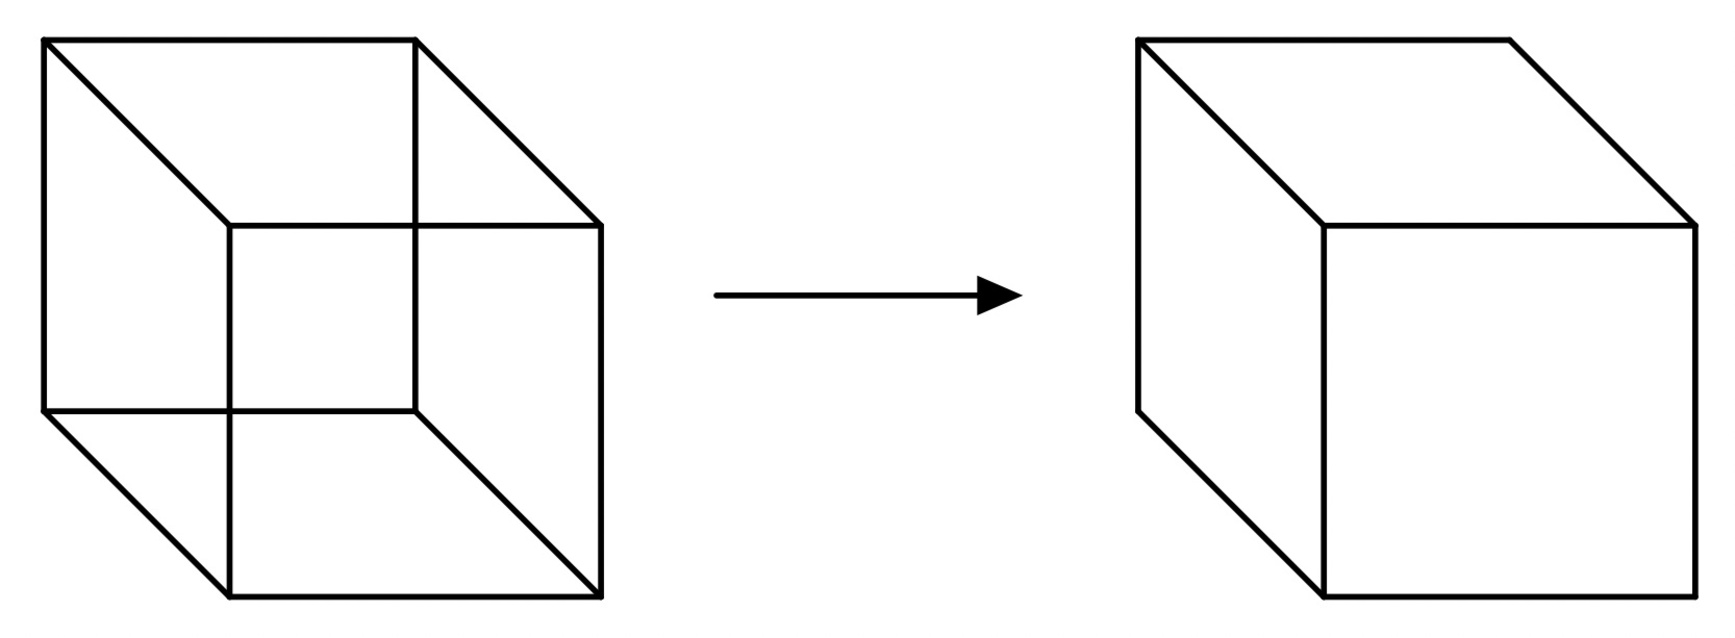
\includegraphics[width=0.65\linewidth]{invis.pdf}
    \caption{Пример удаления невидимых рёбер}
    \label{img:invis}
\end{figure}

Далее будут рассмотрены некоторые алгоритмы удаления невидимых линий и поверхностей.

\subsubsection{Алгоритм, использующий $z$-буфер}
Данный алгоритм считается одним из простейших алгоритмов для удаления невидимых поверхностей \cite{item12}. Алгоритм, использующий $z$-буфер, работает в пространстве изображения. Этот алгоритм основан на идее о буфере кадра, который представляет из себя хранилище информации об интенсивности каждого пиксела в пространстве изображения. Также, в данном алгоритме используется $z$-буфер, хранящий координату $z$ каждого видимого пиксела в пространстве изображения.

Основные этапы работы алгоритма можно описать так:
\begin{enumerate}[label={\arabic*)}]
	\item Буфер кадра заполняется значением, соответствующим фоновому цвету.
	\item $z$-буфер заполняется минимальным значением координаты $z$.
	\item Каждый многоугольник преобразуется в растровую форму, для каждого пиксела многоугольника вычисляется значение координаты $z$.
	\item Если глубина текущего пиксела больше, чем глубина, записанная на соответствующей по координатам $x,\ y$ позиции в $z$-буфере, то записать её на эту позицию и обновить информацию в буфере кадра для данной позиции. Иначе, никаких действий не производится.
\end{enumerate}

Там, где это целесообразно, то есть для невыпуклых многогранников, предварительным шагом будет являться удаление нелицевых граней.

Уравнение плоскости имеет вид $ax + by + cz + d = 0$. Тогда координату $z$ можно выразить так: \begin{equation}
	z = \frac{-(ax + by + d)}{c} \neq 0.
\end{equation}

Для текущей сканирующей строки значение $y$ является постоянным. Тогда для пиксела с координатой $x^{'} = x + \delta x$ глубину можно выразить так: \begin{equation}
	z^{'} - z = -\frac{ax^\prime + d}{c} +\frac{ax + d}{c} = \frac{a(x - x^\prime)}{c}.
\end{equation}

Данная запись эквивалентна записи \begin{equation}
	z^{'} = z - \frac{a}{c}\delta x.
\end{equation}

Учитывая, что пикселы рассматриваются последовательно по сканирующей строке, то есть $\delta x = 1$, формулу можно записать в виде: \begin{equation}
	z^{'} = z - \frac{a}{c}.
\end{equation}

Пример работы алгоритма представлен на рис. \ref{img:z-buf}.

\begin{figure}[h!]
    \centering
    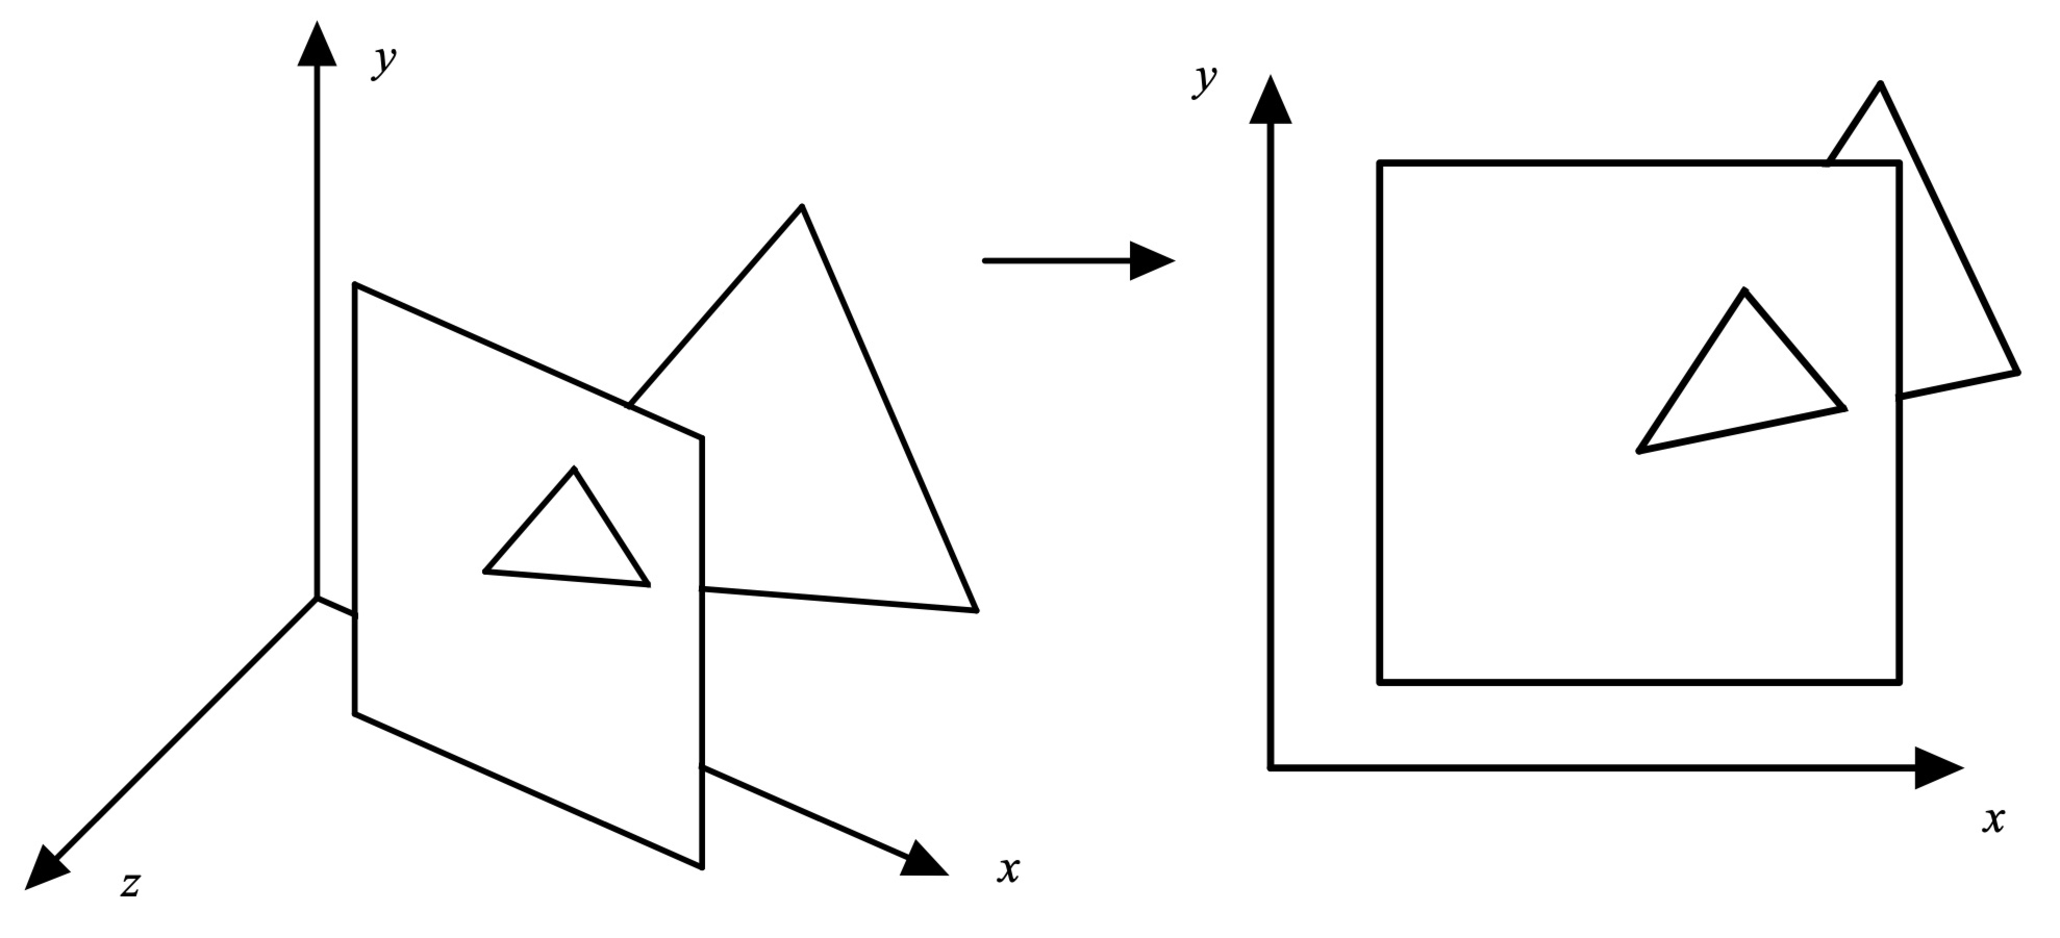
\includegraphics[width=0.9\linewidth]{z-buf.pdf}
    \caption{Пример работы алгоритма, использующего $z$-буфер}
    \label{img:z-buf}
\end{figure}

Свойством данного алгоритма является простота решения им задач визуализации сложных пересечений и удаления невидимых поверхностей \cite{item12}: они не требуют особой обработки и рассматриваются аналогично со всеми остальными ситуациями. Алгоритм, использующий $z$-буфер, допускает построение сцен любой сложности, при этом не требуя предварительной сортировки элементов сцены и обеспечивая линейную оценочную трудоёмкость. К свойствам данного алгоритма также относятся большое потребление ресурсов в теоретической оценке и трудоёмкость устранения лестничного эффекта, реализации эффектов прозрачности и просвечивания. Попытка реализовать данные свойства зачастую приводит к некорректной работе алгоритма. Также, для невыпуклых тел приходится производить дополнительные вычисления, что замедляет работу алгоритма.

\subsubsection{Алгоритмы построчного сканирования}
Данный класс алгоритмов обрабатывает сцену в порядке прохождения по её пикселам сканирующей строкой \cite{item12} и оперируют в пространстве изображения. За счёт работы с растровой развёрткой данные алгоритмы позволяют рассматривать задачу удаления невидимых поверхностей как более тривиальную задачу удаления невидимых линий. 

Сканирующая плоскость определяется точкой положения наблюдателя и сканирующей строкой. Пересечение заданной плоскости и сцены определяет окно, в пределах которого решается задача удаления невидимых линий. Пример расположения сканирующей плоскости изображён на рисунке \ref{img:scan}.

\begin{figure}[h!]
    \centering
    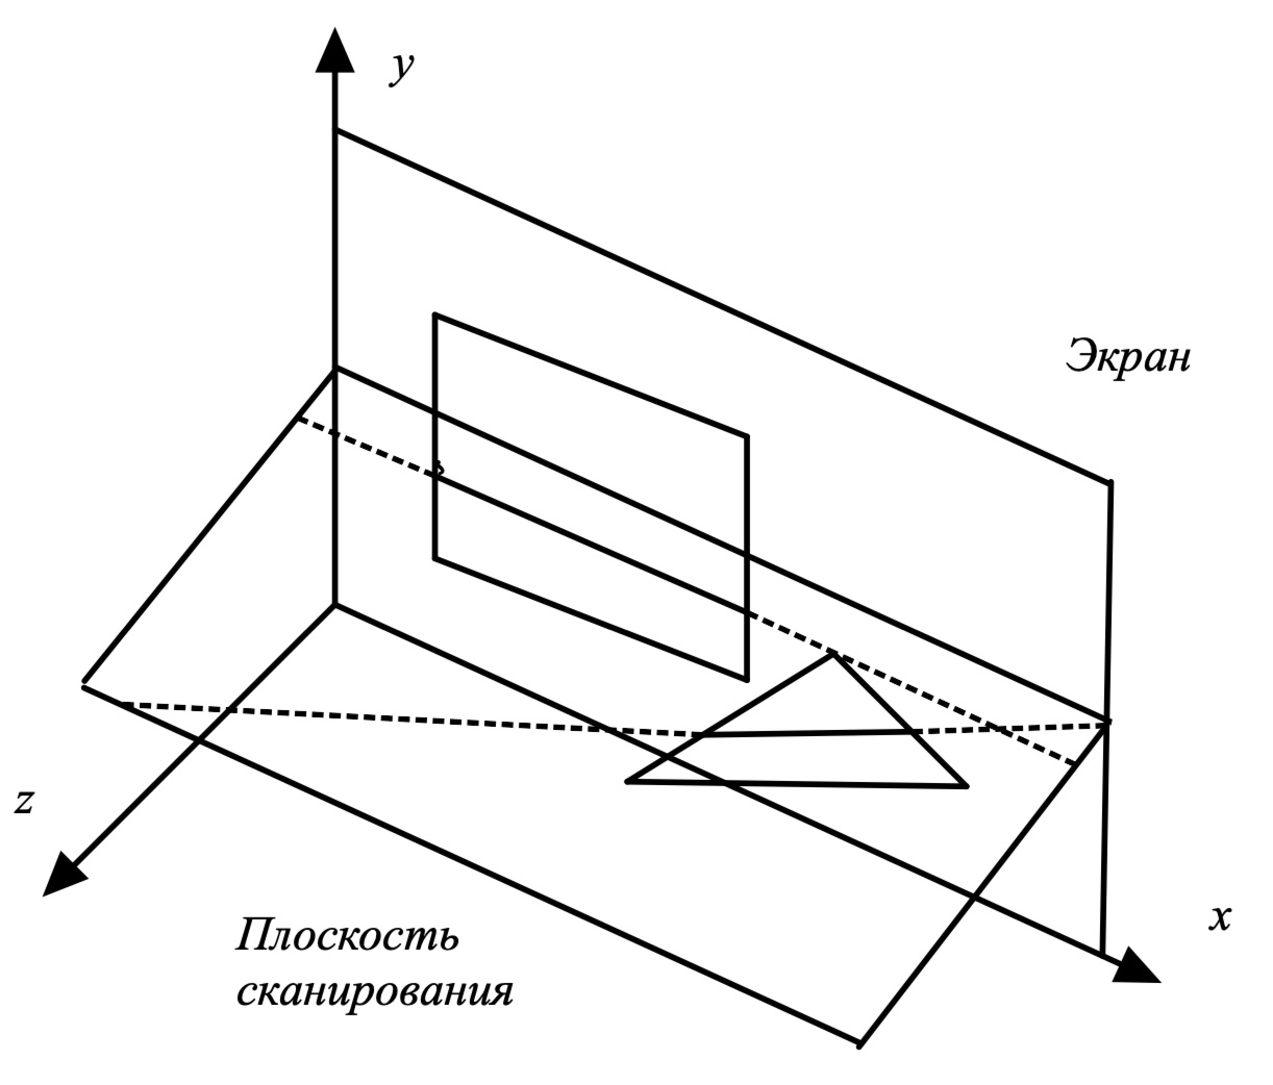
\includegraphics[width=0.6\linewidth]{scan.pdf}
    \caption{Пример расположения сканирующей плоскости}
    \label{img:scan}
\end{figure}

К этому классу алгоритмов относится, например, алгоритм построчного сканирования, использующий $z$-буфер. В отличие от обычного алгоритма $z$-буфера, в этом алгоритма буферы хранятся исключительно для обрабатываемой строки, что улучшает теоретическую оценку потребления ресурсов. Основные этапы работы алгоритма можно описать так:
\begin{enumerate}[label={\arabic*)}]
	\item Для каждой сканирующей строки буфер кадра заполняется значением, соответствующим фоновому цвету, а $z$-буфер~---~минимальным значением координаты $z$.
	\item Определяется пересечение строки с двумерными проекчиями объектов сцены. Пересечения образуют пары.
	\item Глубина каждого пиксела в интервале пары сравневается с глубиной на текущей позиции в $z$-буфере. Если глубина этого пиксела больше, то данный отрезок видим, а соответствующая ему интенсивность заносится в буфер кадра.
	\item Результаты сканирования по строке выводятся на экран слева направо.
\end{enumerate}

Еще одним алгоритмом данного класса является интервальный алгоритм построчного сканирования. В отличие от алгоритма построчного сканирования, использующий $z$-буфер, где вычисление глубины многоугольника происходит на каждом пикселе сканирующей строки, в этом алгоритме строка делится на интервалы точками пересечения рёбер. Это позволяет дополнительно улучшить теоретическую оценку временных затрат.

Некоторые модификации данных алгоритмов позволят также учесть тени, эффект прозрачности и устранить ступенчатость, но не зеркальность поверхности. Также, данные алгоритмы имеют высокую теоретическую оценку по потреблению ресурсов.

\subsubsection{Алгоритм Робертса}
Алгоритм Робертса считается первым известным решением задачи удаления невидимых линий \cite{item12}. Данный алгоритм работает в объектном пространстве и только с выпуклыми телами. Для корректной работы алгоритма должна быть гарантирована возможность представить любое тело как набор пересекающихся плоскостей. В данном алгоритме используются эффективные математические методы, однако его вычислительная трудоёмкость без применения оптимизаций оценивается в $O(n^2)$, где $n$~---~количество объектов сцены, что снижает его «привлекательность». 

Можно выделить четыре основных этапа работы алгоритма:
\begin{enumerate}[label={\arabic*)}]
	\item Подготовка данных. На этом этапе для каждого тела формируется матрица тела, которая далее будет обозначаться как $V$. Любая плоскость может быть задана уравнением вида $ax + by + cz + d = 0$. В матричном виде это можно записать так: \begin{equation} \label{eqn:1} \begin{pmatrix}
			x & y & z & 1
		\end{pmatrix}\begin{pmatrix}
			a & b & c & d
		\end{pmatrix}^{T} = 0. \end{equation}
		Любое тело, по необходимым условиям корректной работы алгоритма, упомянутым выше, может быть представлено как набор пересекающихся плоскостей. Тогда любое тело может быть описано матрицей вида \begin{equation}
		V = \begin{pmatrix}
			a_{1} & a_{2} & \ldots & a_{n}\\
			b_{1} & b_{2} & \ldots & b_{n}\\
			c_{1} & c_{2} & \ldots & c_{n}\\
			d_{1} & d_{2} & \ldots & d_{n}
		\end{pmatrix}.
	\end{equation}
	Любая точка представима в однородных координатах как \begin{equation}
		S = \begin{pmatrix} x, & y, & z, & 1 \end{pmatrix}^{T}.
	\end{equation}
	Если заданная точка принадлежит плоскости, то в результате умножения координат данной точки на вектор коэффициентов уравнения плоскости будет получено нулевое значение, как в (\ref{eqn:1}).
	Иначе, будет получено ненулевое значение, а его знак будет определять, по какую сторону от данной плоскости находится точка. В алгоритме Робертса предполагается, что если точка находится внутри тела, то все произведения координат данной точки на вектора коэффициентов уравнений плоскостей, составляющих это тело, будут положительны. Поэтому зачастую требуется производить коррекцию полученной матрицы, например:
	\begin{equation} \label{eqn:2}
		V = \begin{pmatrix}
			a_{1} & a_{2} \cdot (-1) & a_{3} & a_{4}\\
			b_{1} & b_{2} \cdot (-1) & b_{3} & b_{4}\\
			c_{1} & c_{2} \cdot (-1) & c_{3} & c_{4}\\
			d_{1} & d_{2} \cdot (-1) & d_{3} & d_{4}
		\end{pmatrix}.
	\end{equation} В случае, если для очередной грани условие положительности описанного произведения не выполняется, соответствующий столбец матрицы необходимо умножить на $-1$, что и происходит со вторым столбцом в (\ref{eqn:2}). Для проведения проверки следует взять точку, координаты которой будут получены усреднением всех соответствующих координат вершин данного тела.
	\item Удаление рёбер или граней, экранируемых самим телом. Полагается, что наблюдатель находится в бесконечности на положительной полуоси $z$, а его взгляд направлен в сторону отрицательной полуоси $z$. Тогда вектор взгляда наблюдателя можно задать как \begin{equation}
		E = \begin{pmatrix} 0, & 0, & -1, & 0 \end{pmatrix}^{T}.
	\end{equation}
	Для определения невидимых граней тела, экранируемых самим телом, необходимо умножить вектор $E$ на матрицу данного тела $V$. В результирующем векторе отрицательные компоненты будут соответствовать невидимым граням. Экранируемые рёбра определяются по следующему правилу: невидимые ребра образуются в результате пересечения невидимых граней. Если сцены включает в себя одно тело, работа алгоритма завершается, иначе выполняется следующий этап.
	\item Удаление рёбер или граней, экранируемых другими телами сцены. Пусть наблюдатель находится в точке \begin{equation}
		g = \begin{pmatrix} 0, & 0, & 1, & 0 \end{pmatrix}^{T},
	\end{equation}
	а каждое ребро тел можно задать параметрическим уравнением вида \begin{equation}
		p(t) = p_1 + (p_2 - p_1)t, \quad 0~\le~t~\le~1
	\end{equation}
	где $p_1$ и $p_2$~---~начало и конец ребра соответственно, а $t$~---~параметр. Тогда можно записать уравнение для луча, соединяющего произвольную точку на ребре с точкой, в которой расположен наблюдатель, в виде \begin{equation}
		Q(t, \alpha) = p(t) + \alpha g,
	\end{equation}
	где $p(t)$~---~произвольная точка на данном ребре, а $\alpha$~---~параметр, указывающий расположение точки на заданном луче, причём $\alpha~\ge~0$, что указывает на то, что наблюдатель находится перед телом. Можно составить систему неравенств \begin{equation}
		h_j = QV,
	\end{equation}
	где $h_j > 0,\ j = \overline{1,n}$, а $n$~---~количество граней тела.
	Невидимым точкам ребра $p_1p_2$ соответствуют такие значения параметров $t$ и $\alpha$, при которых выполняются все неравенства системы. Система неравенств задает область допустимых решений. Все точки расположенные внутри области определяют координаты невидимых точек отрезка. Минимальное и максимальное значения параметра $t$ задают координаты начала и конца невидимой части отрезка, поэтому необходимо их вычислить.
	\item Удаление линий пересечения тел, экранируемых самими телами, которым принадлежат эти линии, так как эти тела связаны отношением протыкания, и другими телами. В случае существования отношения протыкания появляются решения на границе $\alpha = 0$. Для этого необходимо запомнить все точки протыкания и добавить к сцене отрезки, образованные путём соединения каждой точки протыкания со всеми остальными точками протыкания для данной пары объектов. Затем проверяется экранирование этих отрезков данными и другими телами. Видимые отрезки образуют структуру протыкания.
\end{enumerate}

На рисунке \ref{img:rob} представлены основные сущности, необходимые для понимания этапов работы алгоритма Робертса.

\begin{figure}[h!]
    \centering
    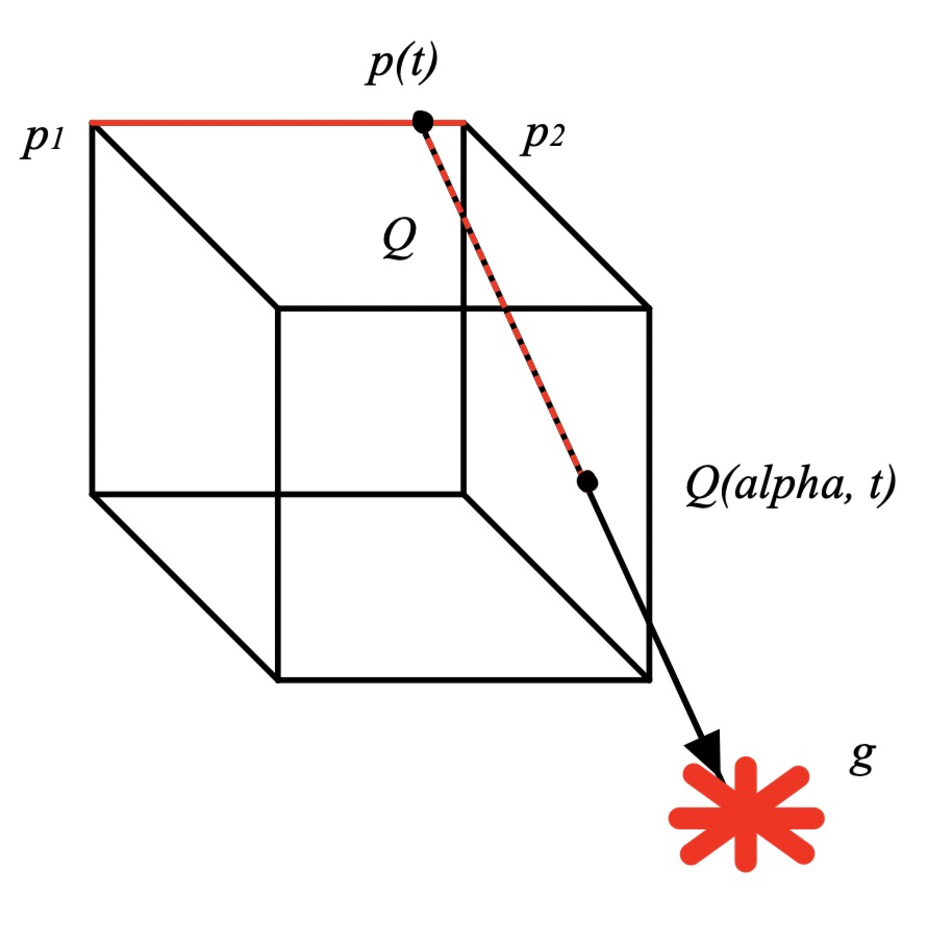
\includegraphics[width=0.4\linewidth]{rob.pdf}
    \caption{Основные сущности, необходимые для понимания этапов работы алгоритма Робертса}
    \label{img:rob}
\end{figure}

Данный алгоритм предоставляет высокую точность вычислений, как и другие алгоритмы, работающие в объектном пространстве, но обладает высокой оценочной сложностью и не позволяет изображать зеркальные поверхности. Также, к недостаткам данного алгоритма можно отнести необходимость дополнительных проверок: на выпуклость тел и на корректность полученных матриц тел. 

Было принято решение не рассматривать другие алгоритмы, работающие в объектном пространстве, как и алгоритм Робертса, так как они имеют схожие свойства и нецелесообразны к использованию для отрисовки сложных сцен.

\subsubsection{Алгоритмы разбиения на окна}
Данные алгоритмы основаны на идее о том, что большая часть времени обработки уходит на анализ областей с высоким информационным содержимым \cite{item12}. То есть производится попытка ускорить обработку сцены за счёт предположения об однородности отдельных достаточно крупных её участков.

Основные этапы можно обобщённо описать так:
\begin{enumerate}[label={\arabic*)}]
	\item Рассматривается окно размером в растр изображения.
	\item Если в окне есть объекты и оно не является достаточно простым для визуализации, то окно разбивается на подокна.
	\item Так происходит до тех пор, пока на данном шаге окно либо не окажется пустым, либо не окажется достаточно простым для визуализации, либо не достигнет предела разрешения, ограниченного точностью растрового дисплея.
	\item В таком случае, информация в окне усредняется, и результат изображается с одинаковой интенсивностью.
\end{enumerate}

Одним из алгоритмов этого класса является алгоритм Варнока. Данный алгоритм работает в пространстве изображения. Основные этапы можно описать так:
\begin{enumerate}[label={\arabic*)}]
	\item Окно, выделяемое по вышеописанному принципу, делится на 4 части, если оно непустое. Окно считается непустым, когда все многоугольники по отношению к нему являются внешними. Критерии расположения многоугольников описаны ниже.
	\item Если все многоугольники сцены являются внешними: окно закрашивается цветом фона. Если внутри окна только один многоугольник: площадь окна вне многоугольника заполняется фоновым цветом, а сам многоугольник заполняется заданным для него цветом.Если окно охвачено ровно одним многоугольником, окно заполняется цветом многоугольника. Если с окном связано несколько многоугольников, но ближе всех прочих к наблюдателю расположен охватывающий, то окно заполняется цветом охватывающего многоугольника. В более сложных случаях проводится разбиение окна.
	\item В случае достижения предела точности определяем глубину каждого из рассматриваемых многоугольников в этой точке. Пиксел закрашивается цветом охватывающего его многоугольника, наиболее близкого относительно центра данного пиксела, либо цветом фона, если для этого пиксела нет охватывающих многоугольников.
\end{enumerate}

Для выпуклых многогранников перед началом работы требуется устранение нелицевых граней.

Способы расположения многоугольников относительно окна:
\begin{itemize}
	\item внешний располагается целиком вне данного окна ($a$ на рис. \ref{img:windows});
	\item внутренний располагается целиком внутри данного окна ($b$ на рис. \ref{img:windows});
	\item пересекающий пересекает границу данного окна ($c$ на рис. \ref{img:windows});
	\item охватывающий полностью заключает данное окно внутри себя ($d$ на рис. \ref{img:windows});
\end{itemize}

\newpage

\begin{figure}[h!]
    \centering
    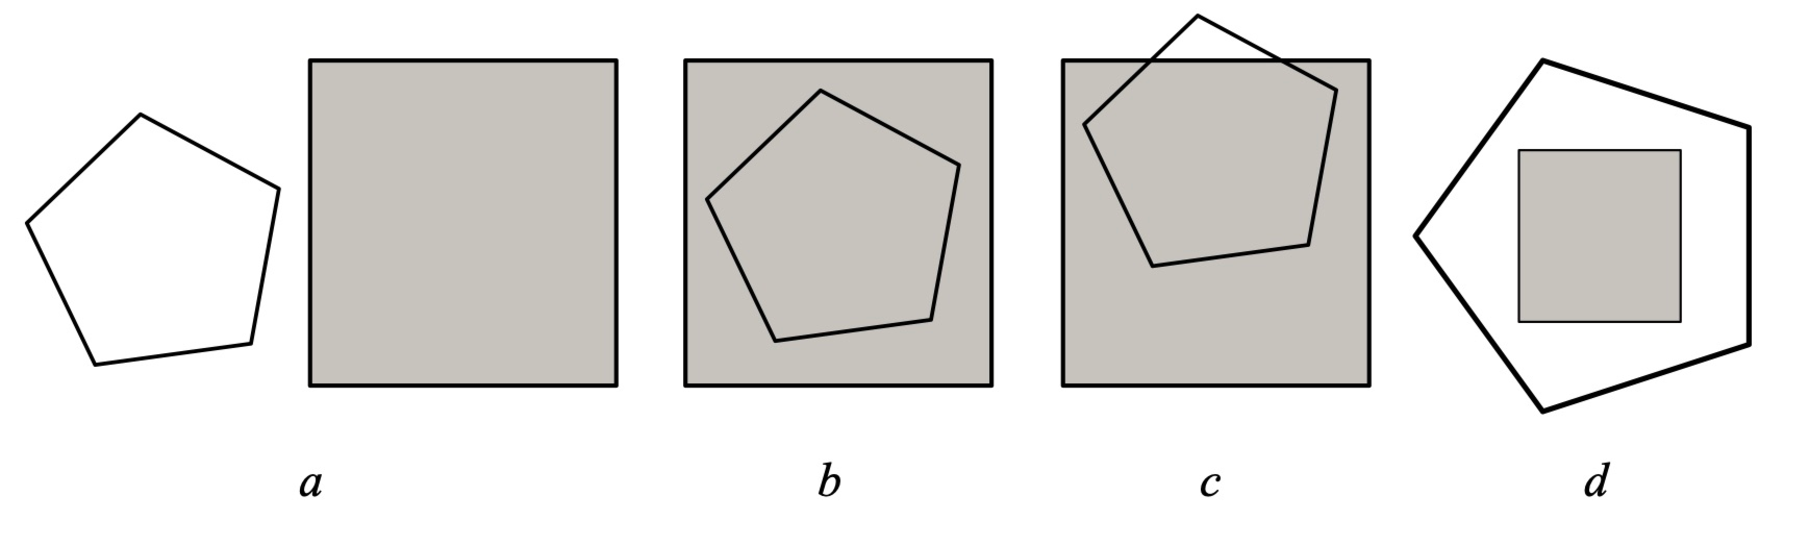
\includegraphics[width=1\linewidth]{windows.pdf}
    \caption{Способы расположения многоугольников относительно окна}
    \label{img:windows}
\end{figure}

Алгоритм Вейлера-Азертона работает немного иначе, осуществляя сортировки по глубине, но так же подразумевает разбиение растра на более мелкие участки. Рассмотрение этого алгоритма, в связи с тем, что он работает в объектом пространстве и нецелесообразен к использованию на сложных сценах, было принято решение не проводить.
%\begin{enumerate}[label={\arabic*)}]
%	\item Производится предварительная сортировка по глубине.
%	\item По границе ближайшего к наблюдателю многоугольника производится отсечение, то есть сортировка многоугольников на плоскости и распределение их по двум спискам~---~внутреннему и внешнему.
%	\item Многоугольники, экранируемые ближайшим к наблюдателю многоугольником, удаляются. Во внутреннем списке остаётся только отсекающий многоугольник.
%	\item При необходимости устранения неопределённостей производится рекурсивное подразбиение и сортировка. Такая ситуация возможно при неполном экранировании какого-либо многоугольника.
%\end{enumerate}
%
%Данный алгоритм работает в объектном пространстве.

Алгоритмы разбиения на окна позволяют устранять ступенчатость при использовании некоторых модификаций, но требуют выполнения большого количества разбиений, что может замедлять работу реализации, и не позволяют учитывать определённые оптические эффекты. Также, некоторые из них, например, алгоритм Варнока, требует проведения дополнительных операций в частных, но достаточно распространённых случаях.

\subsubsection{Алгоритм прямой трассировки лучей}
В отличие от ранее рассмотренных алгоритмов, эффективность алгоритма прямой трассировки лучей не зависит от характеристик сцены, к которой он примяняется \cite{item12}. Это связано с тем, что процесс его работы не учитывает характеристики объектов. Главная идея алгоритма может быть выражена в следующих соображениях:
\begin{enumerate}[label={\arabic*)}]
	\item Из заданных источников света испускаются лучи света.
	\item Лучи света достигают поверхностей объектов и либо преломляются, либо проходят сквозь неё.
	\item Свет доходит до наблюдателя и позволяет ему увидеть объект, через который прошёл или в котором преломился данный луч.
\end{enumerate}

Было установлено, что такая последовательность работы алгоритма будет неэффективна в связи с тем, что немногие лучи света достигнут наблюдателя. Поэтому будет выполнено множество лишних вычислений, из-за чего данный алгоритм практически не используется \cite{item12}. В связи этим он будет исключён из дальнейшего рассмотрения. 

\subsubsection{Алгоритм обратной трассировки лучей}
Алгоритм обратной трассировки лучей работает в пространстве изображения \cite{item12}. Картинная плоскость, т.е. растр, перпендикулярна оси $OZ$. Наблюдатель находится на положительной полуоси $OZ$. При простой трассировке полагается, что наблюдатель расположен в бесконечности, и, соответственно, все световые лучи параллельны оси $z$. При учёте перспективы полагается, что наблюдатель расположен не в бесконечности, и, соответственно, световые лучи необязательно параллельны оси $z$. На рис. \ref{img:trace-inf} изображена простая трассировка луча, а на рис. \ref{img:trace-near} изображена трассировка луча с учётом перспективы.

\begin{figure}[h!]
    \centering
    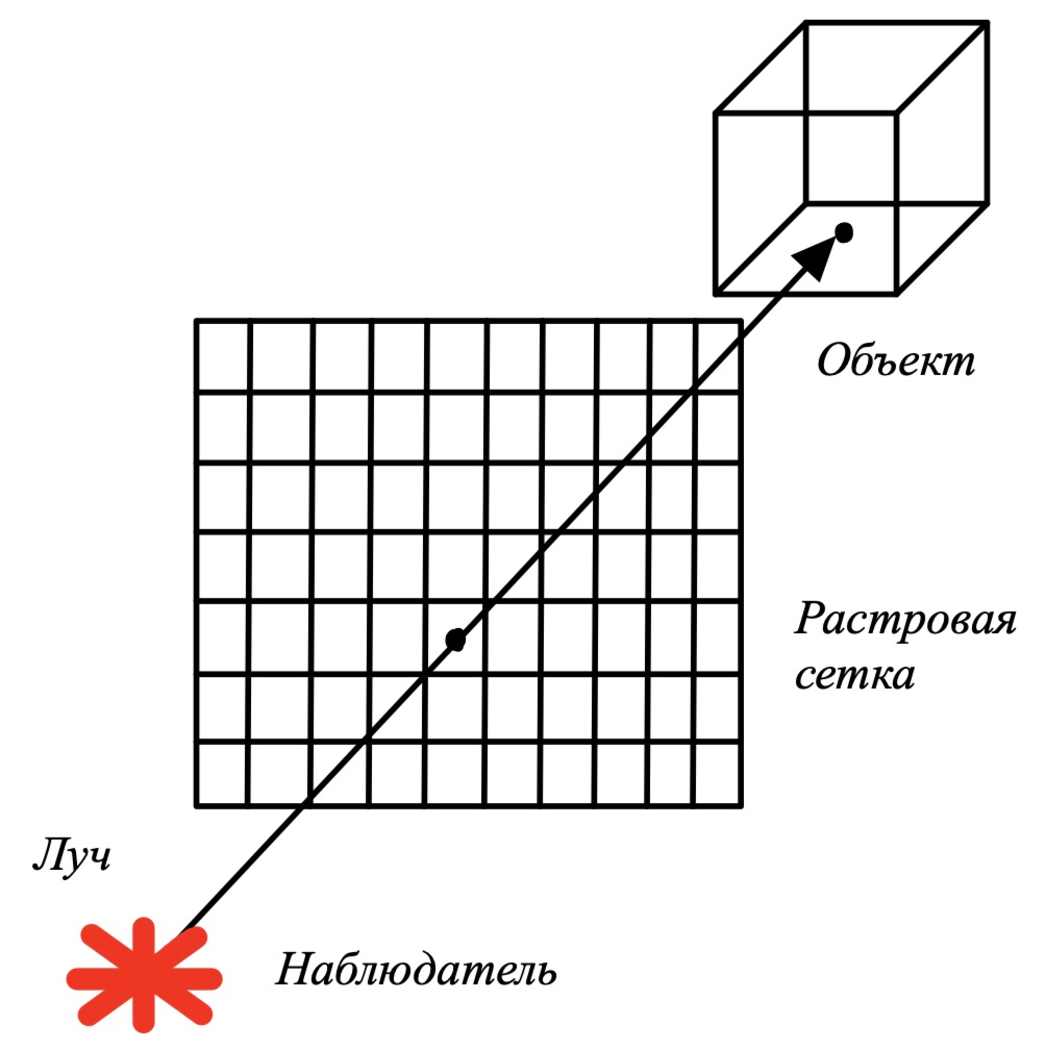
\includegraphics[width=0.4\linewidth]{trace-near.pdf}
    \caption{Простая трассировка луча}
    \label{img:trace-inf}
\end{figure}

\begin{figure}[h!]
    \centering
    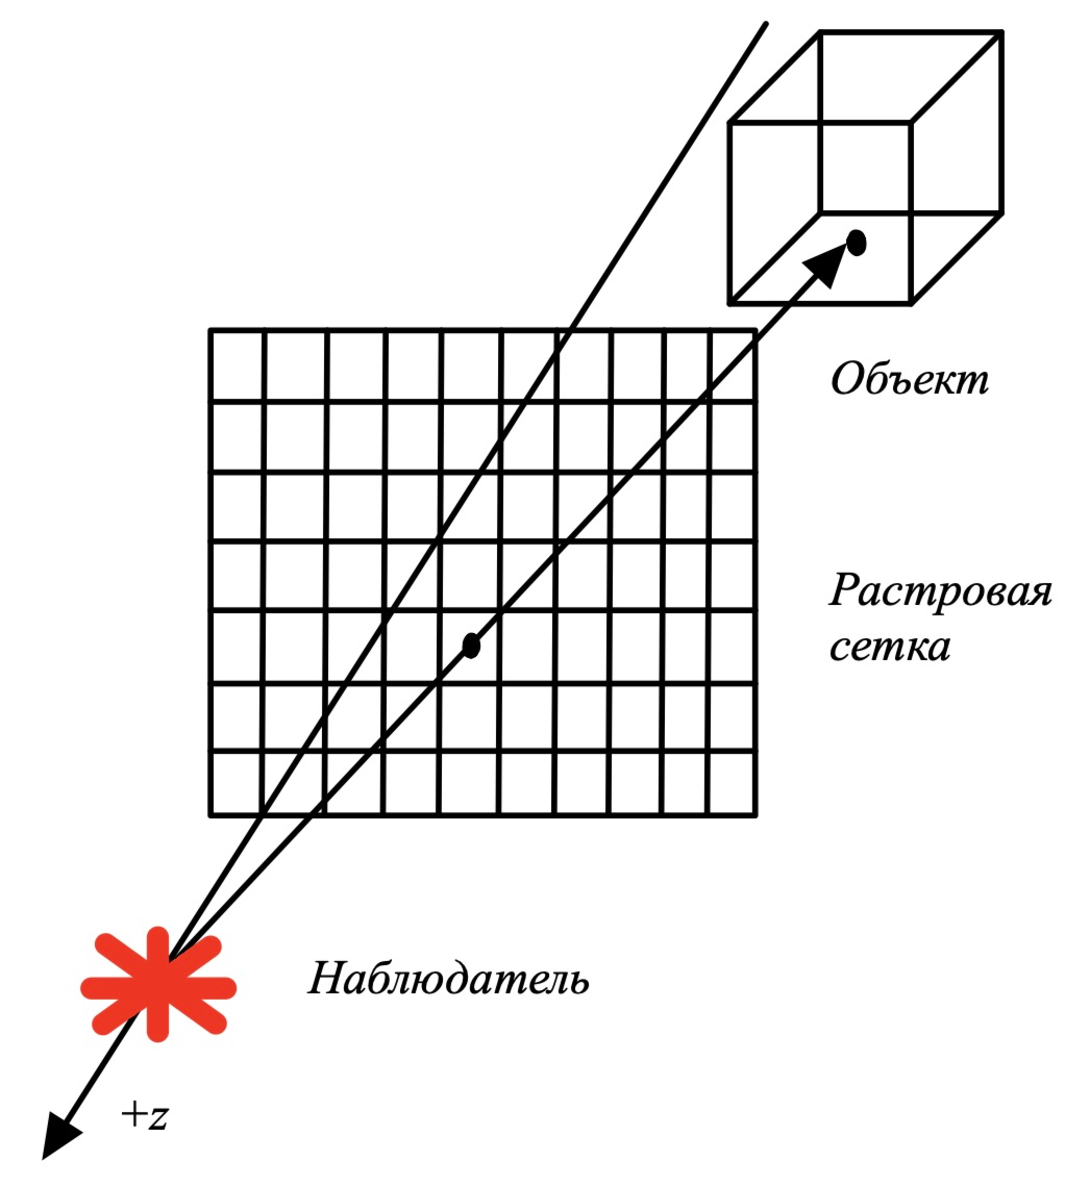
\includegraphics[width=0.4\linewidth]{trace-inf.pdf}
    \caption{Трассировка луча с учётом перспективы}
    \label{img:trace-near}
\end{figure} 

Основные этапы работы алгоритма обратной трассировки лучей:
\begin{enumerate}[label={\arabic*)}]
	\item В каждый пиксел растра последовательно испускаются лучи из положения наблюдателя.
	\item Осуществляется поиск ближайшего к наблюдателю пересечения луча взгляда с объектом сцены. Необходимо проверить пересечение каждого объекта сцены с каждым лучом. Пересечение с максимальным значением $z$ представляет видимую поверхность для данного пиксела.
	\item Для дальнейшего определения цвета пиксела рассматриваются лучи от точки пересечения луча наблюдения с объектом к каждому источнику света. Если на пути к источнику света луч пересекает иной объект, то свет от того источника не учитывается в расчёте цвета данного пиксела. Если для луча от наблюдателя не найдено объектов, с которыми он пересекается, пиксел закрашивается цветом фона.
	\item Для расчёта отражений и преломлений луча, встретившего на своей траектории объект, используются физические законы, например, равенство угла падения и отражения, закон Снеллиуса, рассчитывается направление луча отраженного и преломлённого. Найденная точка пересечения теперь считается точкой наблюдения, и описанный алгоритм испускания луча повторяется столько раз, сколько составляет максимальная глубина рекурсивных погружений.
\end{enumerate}

Алгоритм обратной трассировки лучей подразумевает множество вычислений, поэтому синтез изображения происходит долго. Возможной является многопоточная реализация алгоритма, при которой вычисление цвета каждого пиксела может быть выполнено параллельно. К свойствам данного алгоритма также относятся независимость метода от специфики обрабатываемого объекта, относительная простота встраивания учёта эффектов отражения одного объекта от другого, преломления, прозрачности, затенения и устранения лестничного эффекта. С этим связана высокая реалистичность получаемого изображения.

\subsubsection{Сравнение рассмотренных алгоритмов удаления невидимых линий и поверхностей}
Для наглядности сравнения рассмотренных алгоритмов удаления невидимых линий и поверхностей с учётом поставленных задач была составлена таблица \ref{table:cmp_algs}. Принятые обозначения: ЗБ~---~алгоритм, использующий $z$-буфер, ПС~---~алгоритмы построчного сканирования, Р~---~алгоритм Робертса, РО~---~алгоритмы разбиения на окна, ОТ~---~алгоритм обратной трассировки лучей, $w$~---~ширина растра, $h$~---~высота растра, $n$~---~количество объектов сцены.

\begin{table}[H]
	\begin{center}
		\caption{\label{table:cmp_algs} Таблица сопоставления рассмотренных алгоритмов удаления невидимых линий и поверхностей}
		\begin{tabular}{
    |c
    |S[table-format=1.0]
    |S[table-format=1.0]
    |S[table-format=1.0]
    |S[table-format=1.0]
    |S[table-format=1.0]|
    }
			\hline
			{\specialcell{\\Свойство\\}} & \multicolumn{5}{c|}{\specialcell{Алгоритм или \\класс алгоритмов}}\\ 
			\cline{2-6}
			&{ЗБ}&{ПС}&{Р}&{РО}&{ОТ}\\ 
		
			\hline
%			{\specialcell{Теоретическая сложность реализации алгоритма}} & Нет & Нет & Да & Нет & Нет & Нет \\ \hline
			{\specialcell{Теоретическая оценка \\потребления ресурсов}} & {\specialcell{$O(w \cdot h)$}} & {\specialcell{$O(w)$}} & {\specialcell{$O(n)$}} & {\specialcell{$O(\log_{} {(w \cdot h)})$}} & {\specialcell{$O(1)$}} \\ \hline
			{\specialcell{Необходимость объёмных \\дополнительных или\\«лишних» вычислений \\в частных случаях}} & Нет & Нет & Да & Да & Нет \\ \hline
			{\specialcell{Возможность учёта всех \\оптических эффектов\\(отражение света, \\преломление света, \\тени и т.д.)}} & Нет & Нет & Нет & Нет & Да \\ \hline
			{\specialcell{Применимость к \\сложным сценам}} & Да & Да & Нет & Да & Да \\ \hline
			{\specialcell{Теоретическая оценка \\эффективности по\\времени}} & {\specialcell{$O(w \cdot h \cdot n)$}} & {\specialcell{$O(w \cdot h \cdot n)$}} & {\specialcell{$O(n^2)$}} & {\specialcell{$O(w \cdot h \cdot n)$}} & {\specialcell{$O(w \cdot h \cdot n)$}} \\ \hline
			
		\end{tabular}
	\end{center}
\end{table}

Оценки сложности в приведённой таблице сформированы на основе данных из источников \cite{item12} и \cite{item13}.Таким образом, так как алгоритм обратной трассировки лучей наилучшим образом удовлетворяет поставленным задачам, именно этот алгоритм был выбран для реализации программы.

\subsection{Задача учёта теней на синтезируемом пространстве для заданного положения наблюдателя}
Для заданного положения наблюдателя на видимой части изображения появляются тени в случае, когда положение наблюдателя не совпадает с положением единственного источника света. Иначе, теней не видно. Тень состоит из двух частей~---~полной тени и полутени \cite{item12}. В машинной графике в основном рассматриваются только точечные источники света, создающие только полную тень, так как в ином случае вычислительные затраты резко возрастут. Если источник светы находится в бесконечности, тени определяются при помощи ортогонального проецирования, иначе~---~с помощью перспективной проекции. Процедура определения теней состоит в том, чтобы условно второй раз произвести действие по определению невидимых поверхностей, но уже не относительно наблюдателя, а относительно каждого источника света. Обобщённая схема процесса определения теней проилюстрирована рис. \ref{img:shadow}.

\begin{figure}[h!]
    \centering
    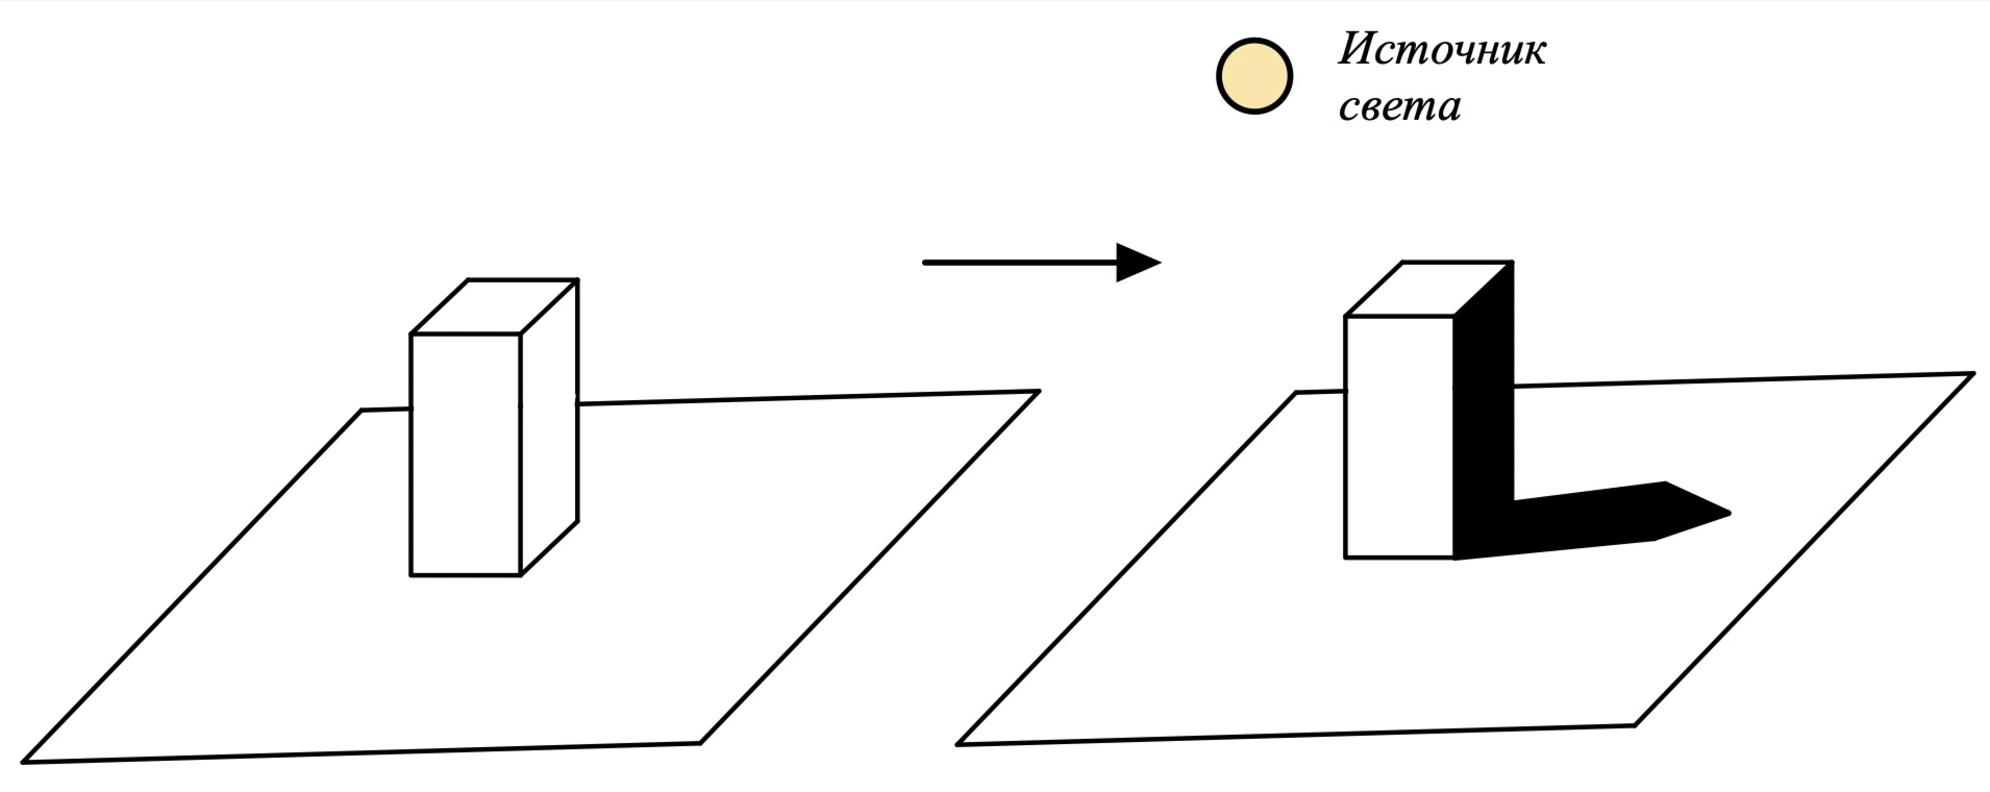
\includegraphics[width=0.8\linewidth]{shadow.pdf}
    \caption{Обобщённая схема процесса определения теней}
    \label{img:shadow}
\end{figure}

В качестве алгоритма удаления невидимых поверхностей был выбран алгоритм обратной трассировки лучей. В этом алгоритме определение теней происходит в процессе работы алгоритма. Если луч, испущенный из точки пересечения луча наблюдения с каким-либо объектом к источнику света, встречает на своём пути иные объекты, то свет от этого источника не доходит до данного пиксела, поэтому он находится в тени относительно этого источника света. Иначе, свет от этого источника будет учтён при отрисовке данного пиксела. Трассировка лучей с построением теней проиллюстрирована рис. \ref{img:trace-shad}.

\begin{figure}[h!]
    \centering
    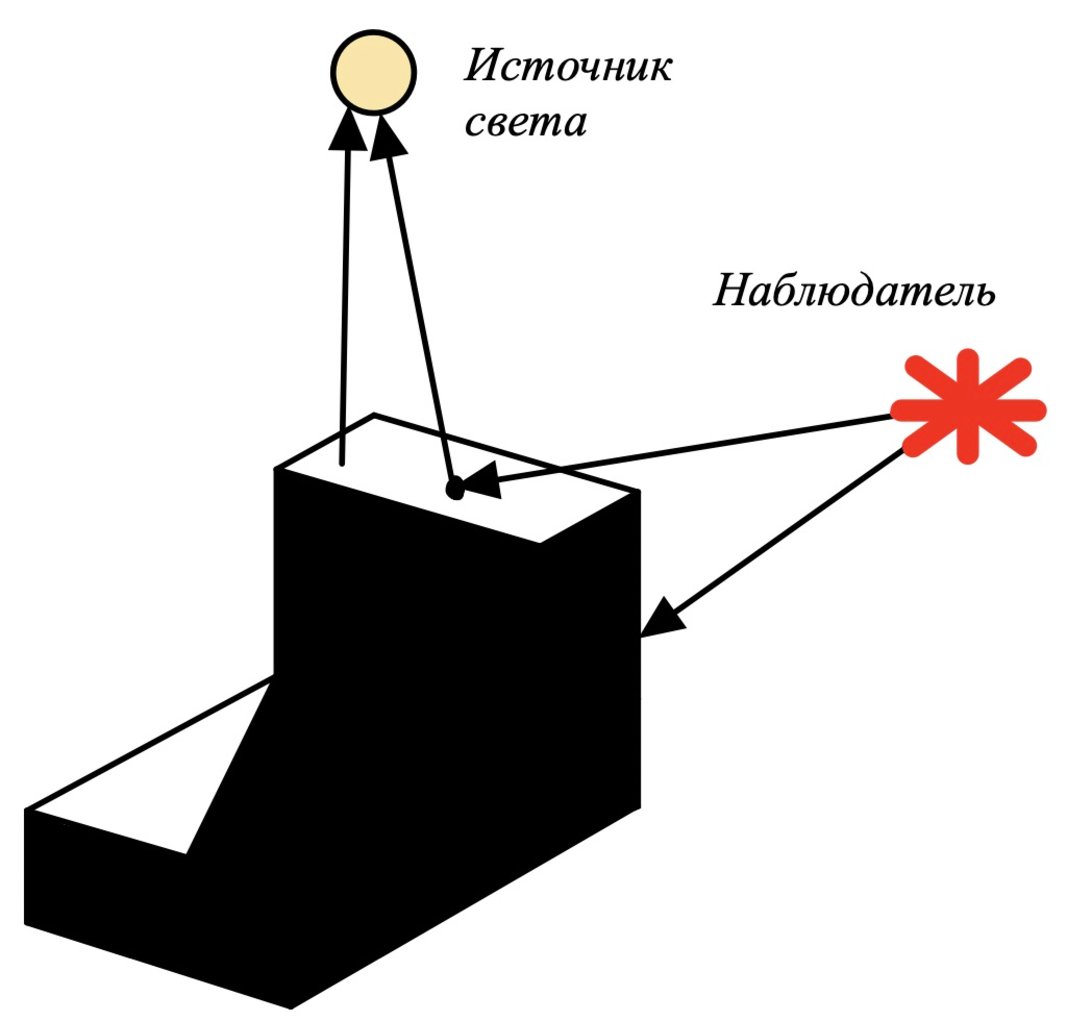
\includegraphics[width=0.35\linewidth]{trace-shad.pdf}
    \caption{Трассировка лучей с построением теней}
    \label{img:trace-shad}
\end{figure}

\subsection{Задача учёта освещения на синтезируемом пространстве для заданного положения наблюдателя}
Для учёта освещенности на видимой части изображения необходимо выбрать используемую модель освещения. Она может быть локальной, что означает учёт только света от источников и ориентации поверхности, или глобальной, что означает также учёт света, отражённого от других объектов или прошедшего сквозь них. Общая схема работы глобальной модели освещения изображена на рис. \ref{img:glob}, причём подразумевается, что на сцене есть тела с зеркальной и прозрачной поверхностями.

\begin{figure}[h!]
    \centering
    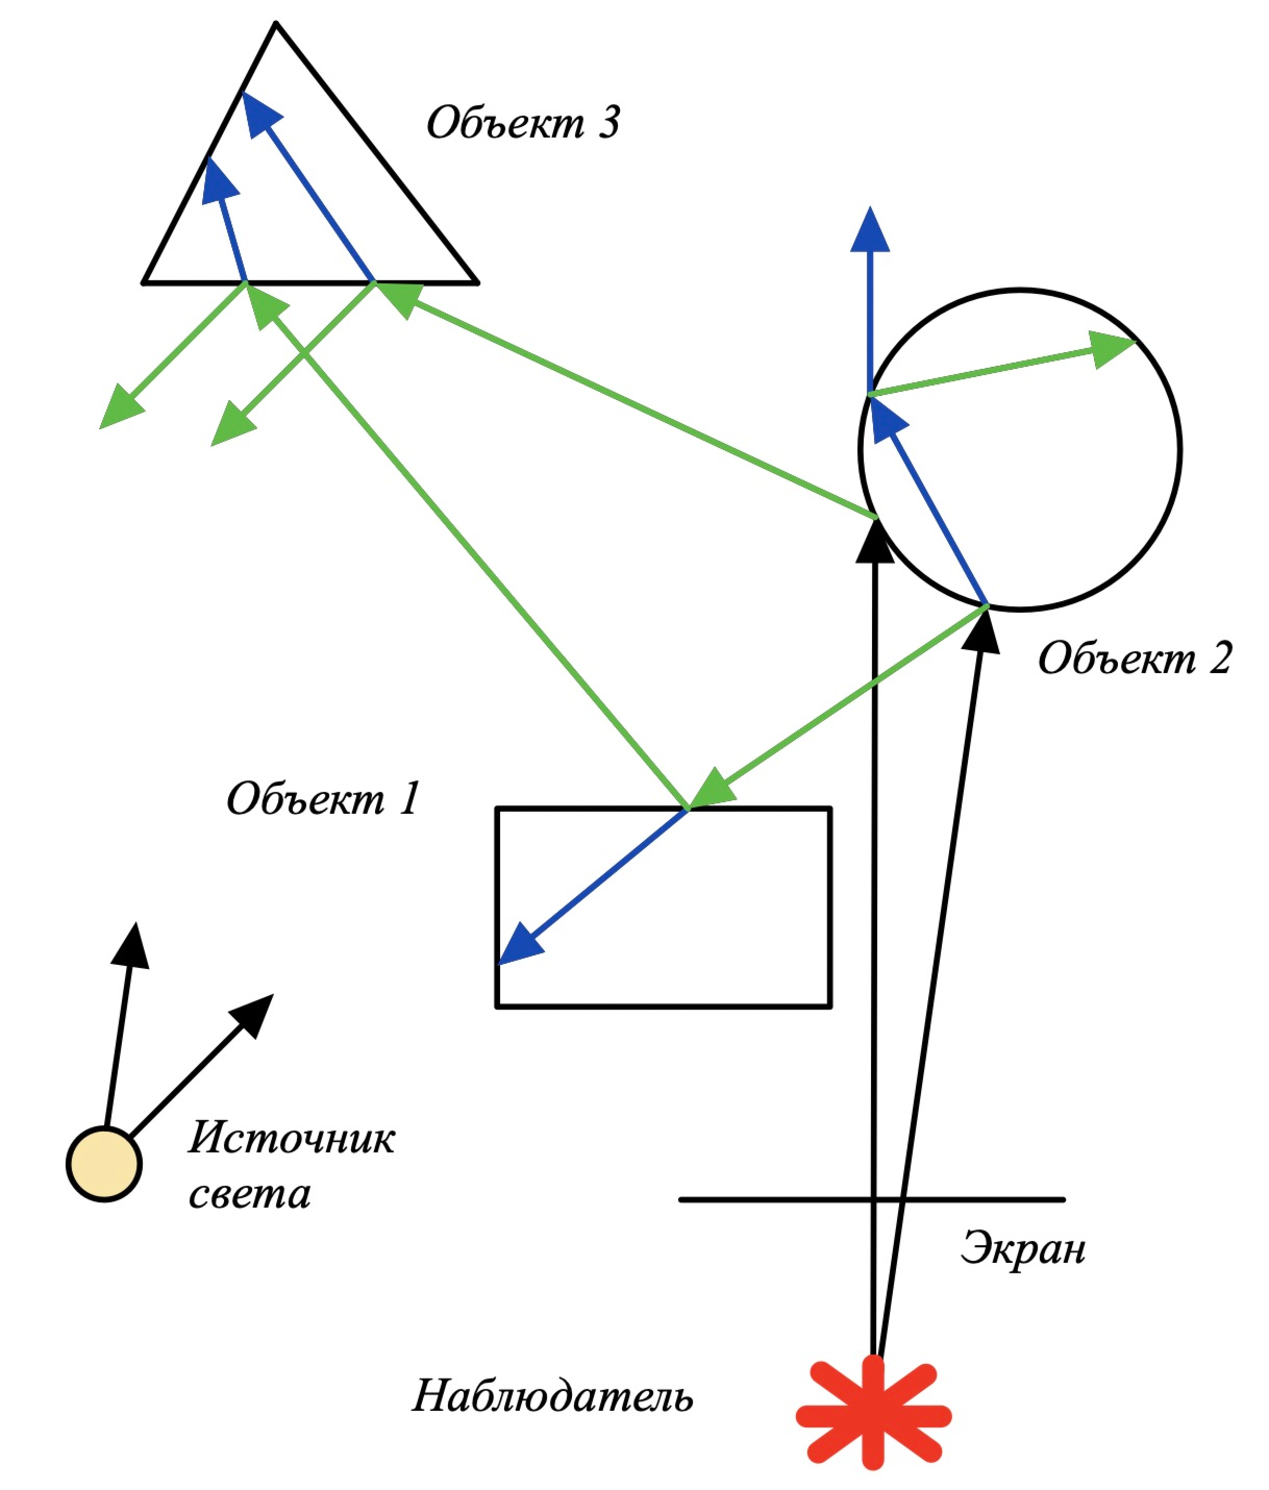
\includegraphics[width=0.45\linewidth]{glob.pdf}
    \caption{Общая схема работы глобальной модели освещения}
    \label{img:glob}
\end{figure}

Используя глобальную модель освещения, можно добиться высокой реалистичности изображения, что в большей степени соответствует поставленным задачам. Только использование алгоритма обратной трассировки лучей позволяет применить глобальную модель освещения в связи с тем, что не исключает из рассмотрения невидимые для наблюдателя грани и позволяет учесть их при отражении и преломлении световых лучей. Таким образом, в данной работе будет использоваться глобальная модель освещения.

При использовании глобальной модели освещения для каждого пиксела изображения определяется его интенсивность. Рассчитываются несколько составляющих интенсивности:
\begin{itemize}
	\item $ambient$~---~фоновое освещение. Постоянно, учитывается для любого участка сцены и не зависит от пространственных координат освещаемой точки и источника;
	\item $diffuse$~---~рассеянный свет. Рассчитывается, как в модели Ламберта по закону косинусов (закону Ламберта): \begin{equation}
		I_d = k_d\cos (L, N)i_d = k_d(L \cdot N)i_d,
	\end{equation}
	где $I_d$~---~рассеянная составляющая освещенности в точке, $k_d$~---~свойство материала воспринимать рассеянное освещение, $L$~---~направление из точки на источник, $N$~---~вектор нормали в точке, $i_d$~---~мощность рассеянного освещения;
	\item $specular$~---~зеркальная составляющая освещения. Зависит от того, насколько близко (насколько мал угол) находятся вектор отражённого луча и вектор к наблюдателю. Учёт этой составляющей представляет собой работу с моделью Фонга~---~комбинацию модели Ламберта и зеркальной составляющей. Так, кроме равномерного освещения на материале при определённых условиях будет появляться блик. Расположение блика на объекте определяется из закона равенства углов падения и отражения. Падающий луч, отраженный луч и нормаль к отражающей поверхности в точке падения лежат в одной плоскости. Нормаль делит угол между лучами на две равные части. Таким образом, отраженная составляющая освещенности в данной точке зависит от величины угла между направлением на наблюдателя и отраженным лучом. Эту зависимость можно выразить следующей формулой: \begin{equation}
		I_s = k_s\cos^{\alpha} (R, V)i_s = k_s(R \cdot V)^{\alpha}i_s,
	\end{equation}
	где $I_s$~---~зеркальная составляющая освещенности в точке,$k_s$~---~коэффициент зеркального отражения,$R$~---~направление отраженного луча,$V$~---~направление на наблюдателя,$i_s$~---~мощность зеркального освещения, $\alpha$~---~коэффициент блеска, свойство материала;
	\item $refract$~---~составляющая интенсивности от преломлённого луча.
\end{itemize}

Обобщая все эти составляющие и учитывая наличие на сцене других тел, можно записать формулу для глобальной модели освещения:
\begin{equation}
	I = k_aI_a + k_d\sum\limits_{j}^{}I_j(N \cdot L_j) + k_s\sum\limits_{j}^{}I_j(V \cdot R_j)^{\alpha}+k_sI_s+k_rI_r,
\end{equation}
где \begin{itemize}
	\item $k_a$ -- коэффициент фонового освещения;
	\item $k_d$ -- коэффициент диффузного отражения;
	\item $k_s$ -- коэффициент зеркального отражения;
	\item $k_r$ -- коэффициент пропускания;
	\item $N$ -- единичный вектор нормали к поверхности в данной точке;
	\item $L_j$ -- единичный вектор, направленный к $j$-му источнику света;
	\item $V$ -- единичный вектор, направленный на наблюдателя;
	\item $R_j$ -- вектор направления отражённого луча $L_j$;
	\item $I_a$ -- интенсивность фонового освещения;
	\item $I_j$ -- интенсивность $j$-го источника света;
	\item $I_s$ --  интенсивность от зеркально отражённого луча;
	\item $I_r$ -- интенсивность от преломлённого луча.
\end{itemize}

В глобальной модели освещения трассировка луча не прекращается при первом найденном пересечении с каким-либо объектом: необходима дальнейшая трассировка отражённого и преломлённого лучей, ход которых рассчитывается по законам геометрической оптики. Процесс продолжается до тех пор, пока очередные лучи не перестанут пересекаться с какими-либо объектами сцены. Такой процесс может стать бесконечным, если задана сложная сцена, поэтому необходимо задать максимальную глубину рекурсии для трассировки.

\section{Физические основы синтеза изображения мыльного пузыря}
В данной работе необходимо получить реалистичное изображение мыльного пузыря. На поверхности мыльного пузыря обычно появляются радужные пятна. Это связано с явлением интерференции света.

Пузырь представляет из себя два мыльных слоя, между которыми заключён слой воды, а внутри находится воздух. Тогда при попадании луча света на поверхность пузыря часть света отражается от первого мыльного слоя, а часть проходит внутрь плёнки, преломляясь, и впоследствии вновь отражаясь от внутреннего мыльного слоя, и снова выходит наружу. При каждом проходе световая волна смещается на определенное значение, пропорциональное длине волны и зависящее от толщины мыльной пленки. Этот процесс показан на рисунке \ref{img:int1}.

\newpage

\begin{figure}[h!]
    \centering
    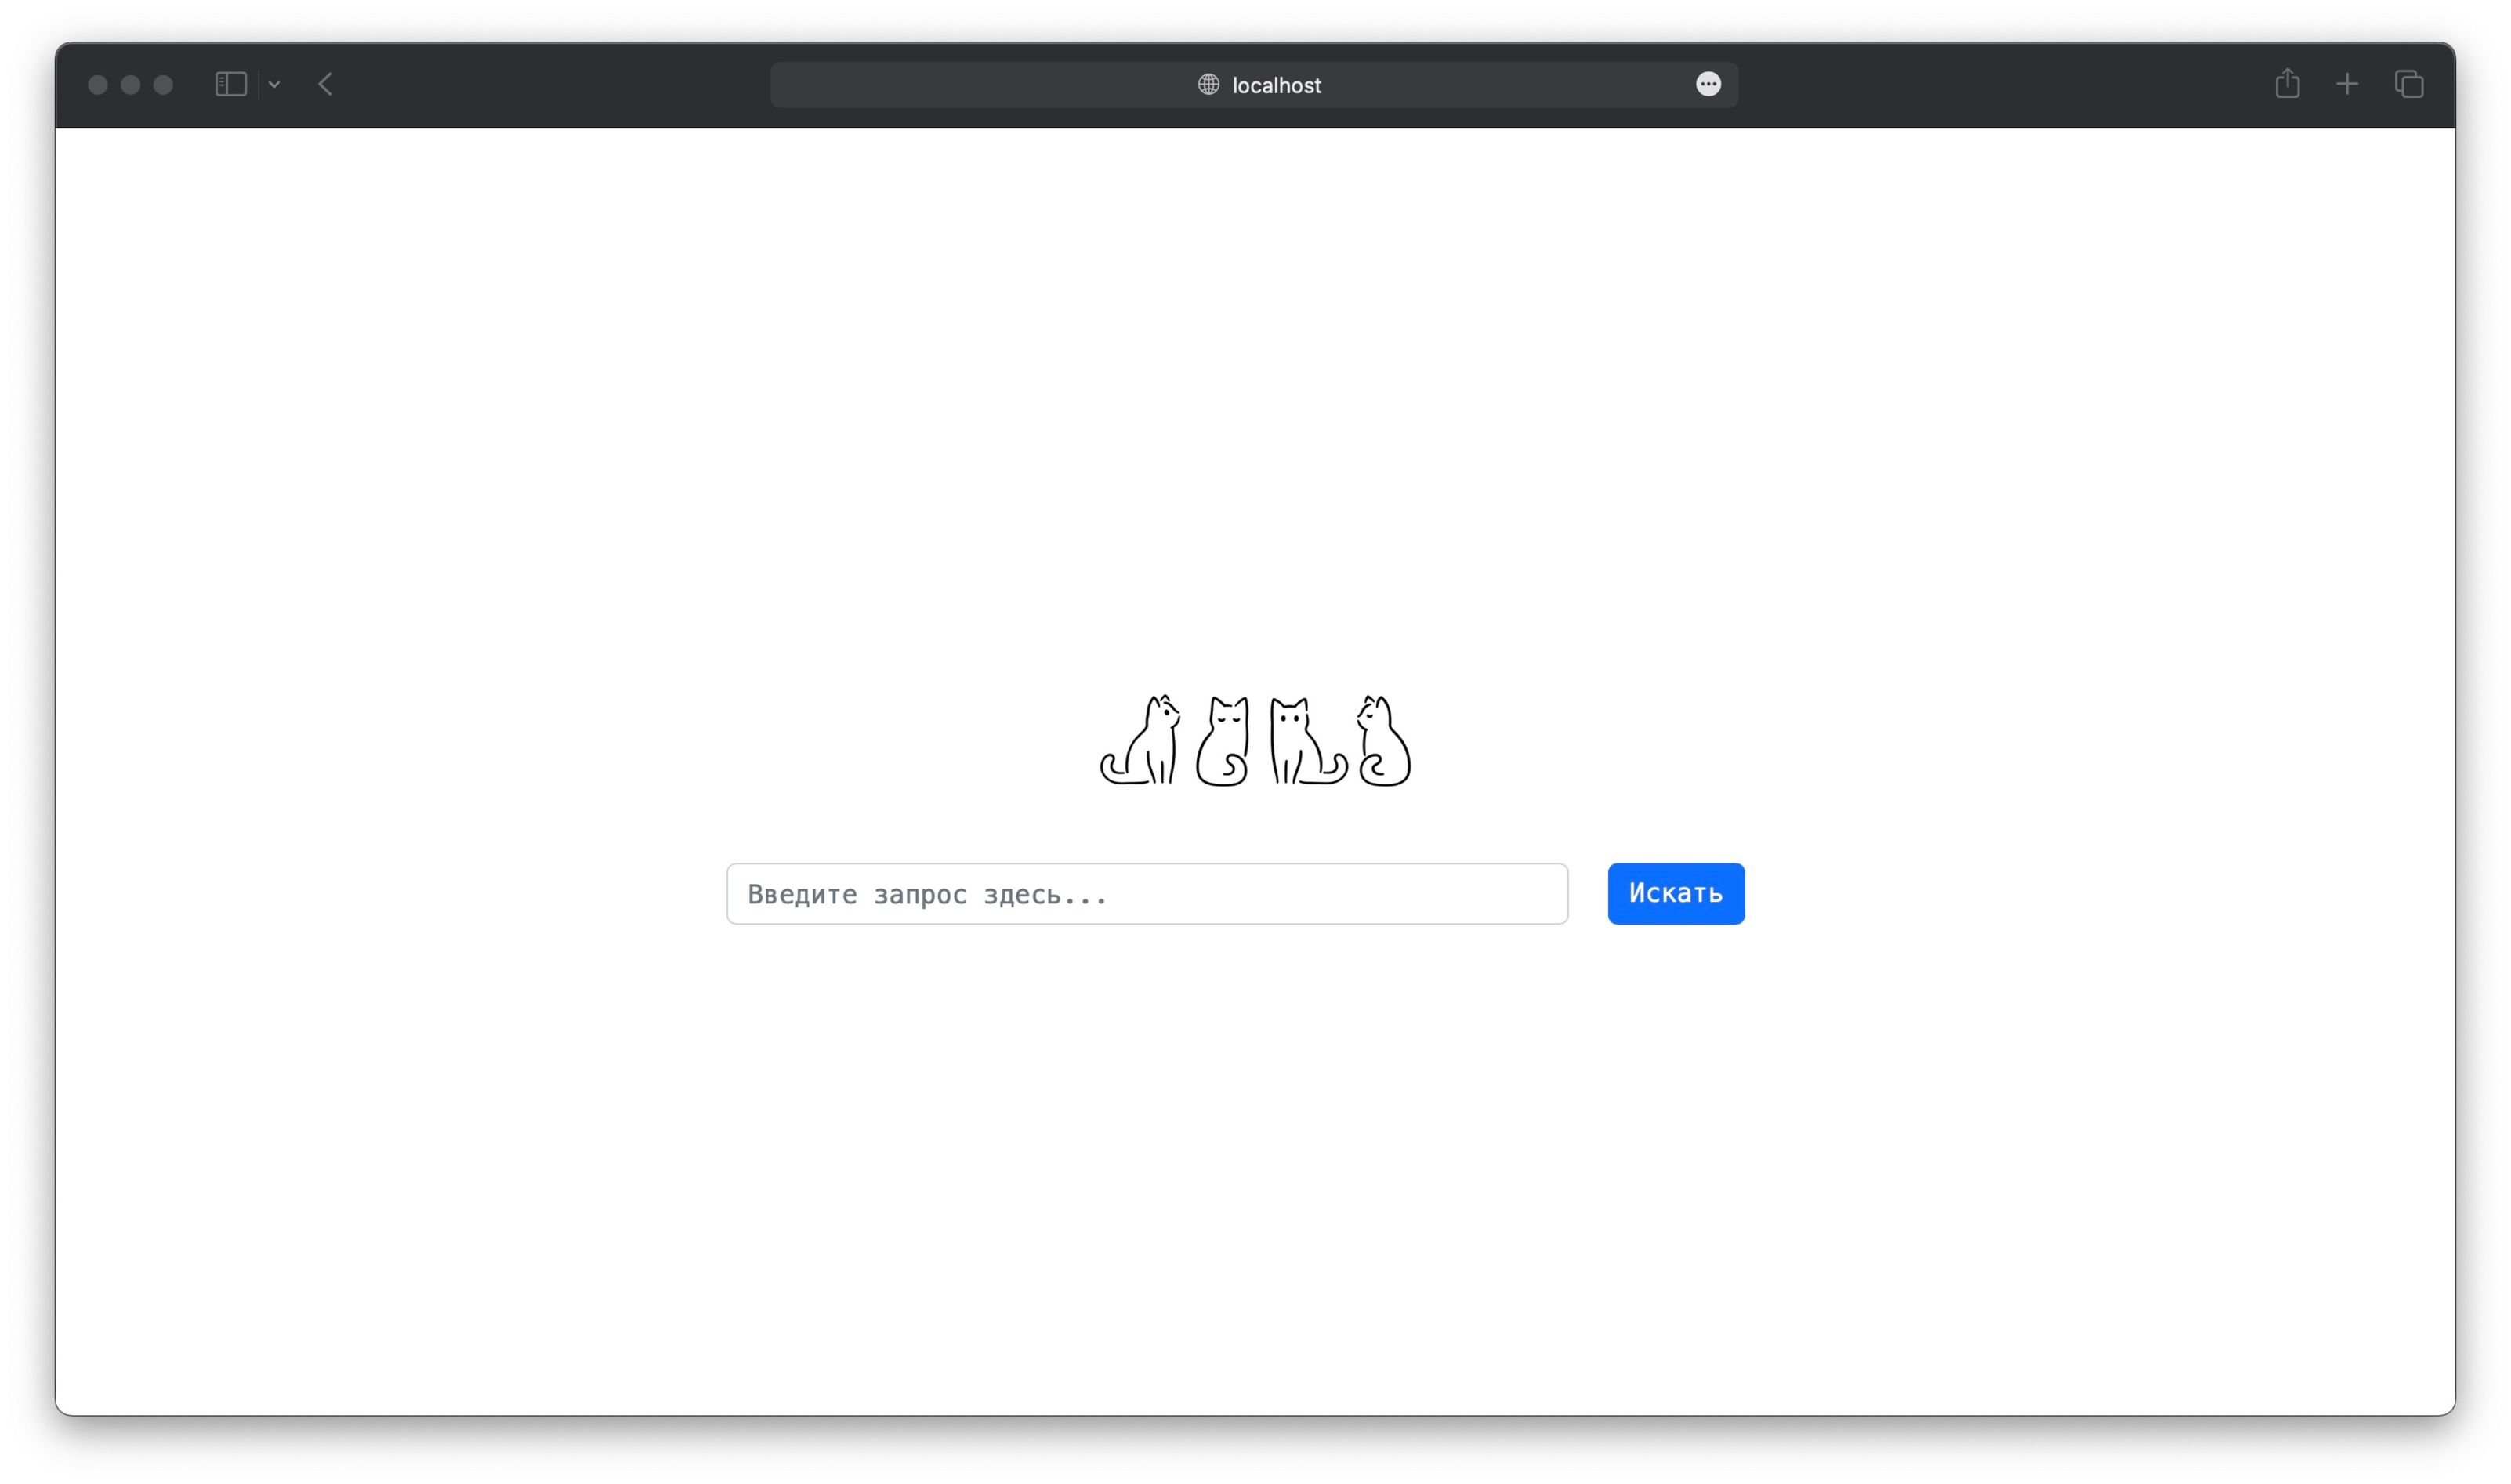
\includegraphics[width=0.37\linewidth]{int1.pdf}
    \caption{Преломление и отражение света в мыльной пленке}
    \label{img:int1}
\end{figure}

Важным свойством мыльной плёнки является то, что вновь вылетевший из плёнки луч $T_3$ параллелен отражённому лучу $R$. Таким образом, свет, движущийся по $R$, будет взаимодействовать со светом на $T_3$. Так как свет~---~это волна, его итоговая интенсивность будет зависеть от длины волны и фазы каждой составляющей волны. Пусть свет, поступающий вдоль $I$ имеет длину волны $\lambda$. Пленка имеет толщину $w$, а показатель преломления пленки равен $\eta$. Угол падения между $I$ и нормалью $N$ к поверхности равен $\theta_i$, а угол преломления~---~$\theta_t$. Свет по лучу $T_3$ будет сдвинут по фазе относительно света по лучу $R$, а разность фаз будет определять, усиливают или гасят эти волны друг друга. Чтобы найти разность фаз, нужно сначала найти оптическую разность хода. Теперь будет рассматриваться рисунок \ref{img:int2}.

\begin{figure}[h!]
    \centering
    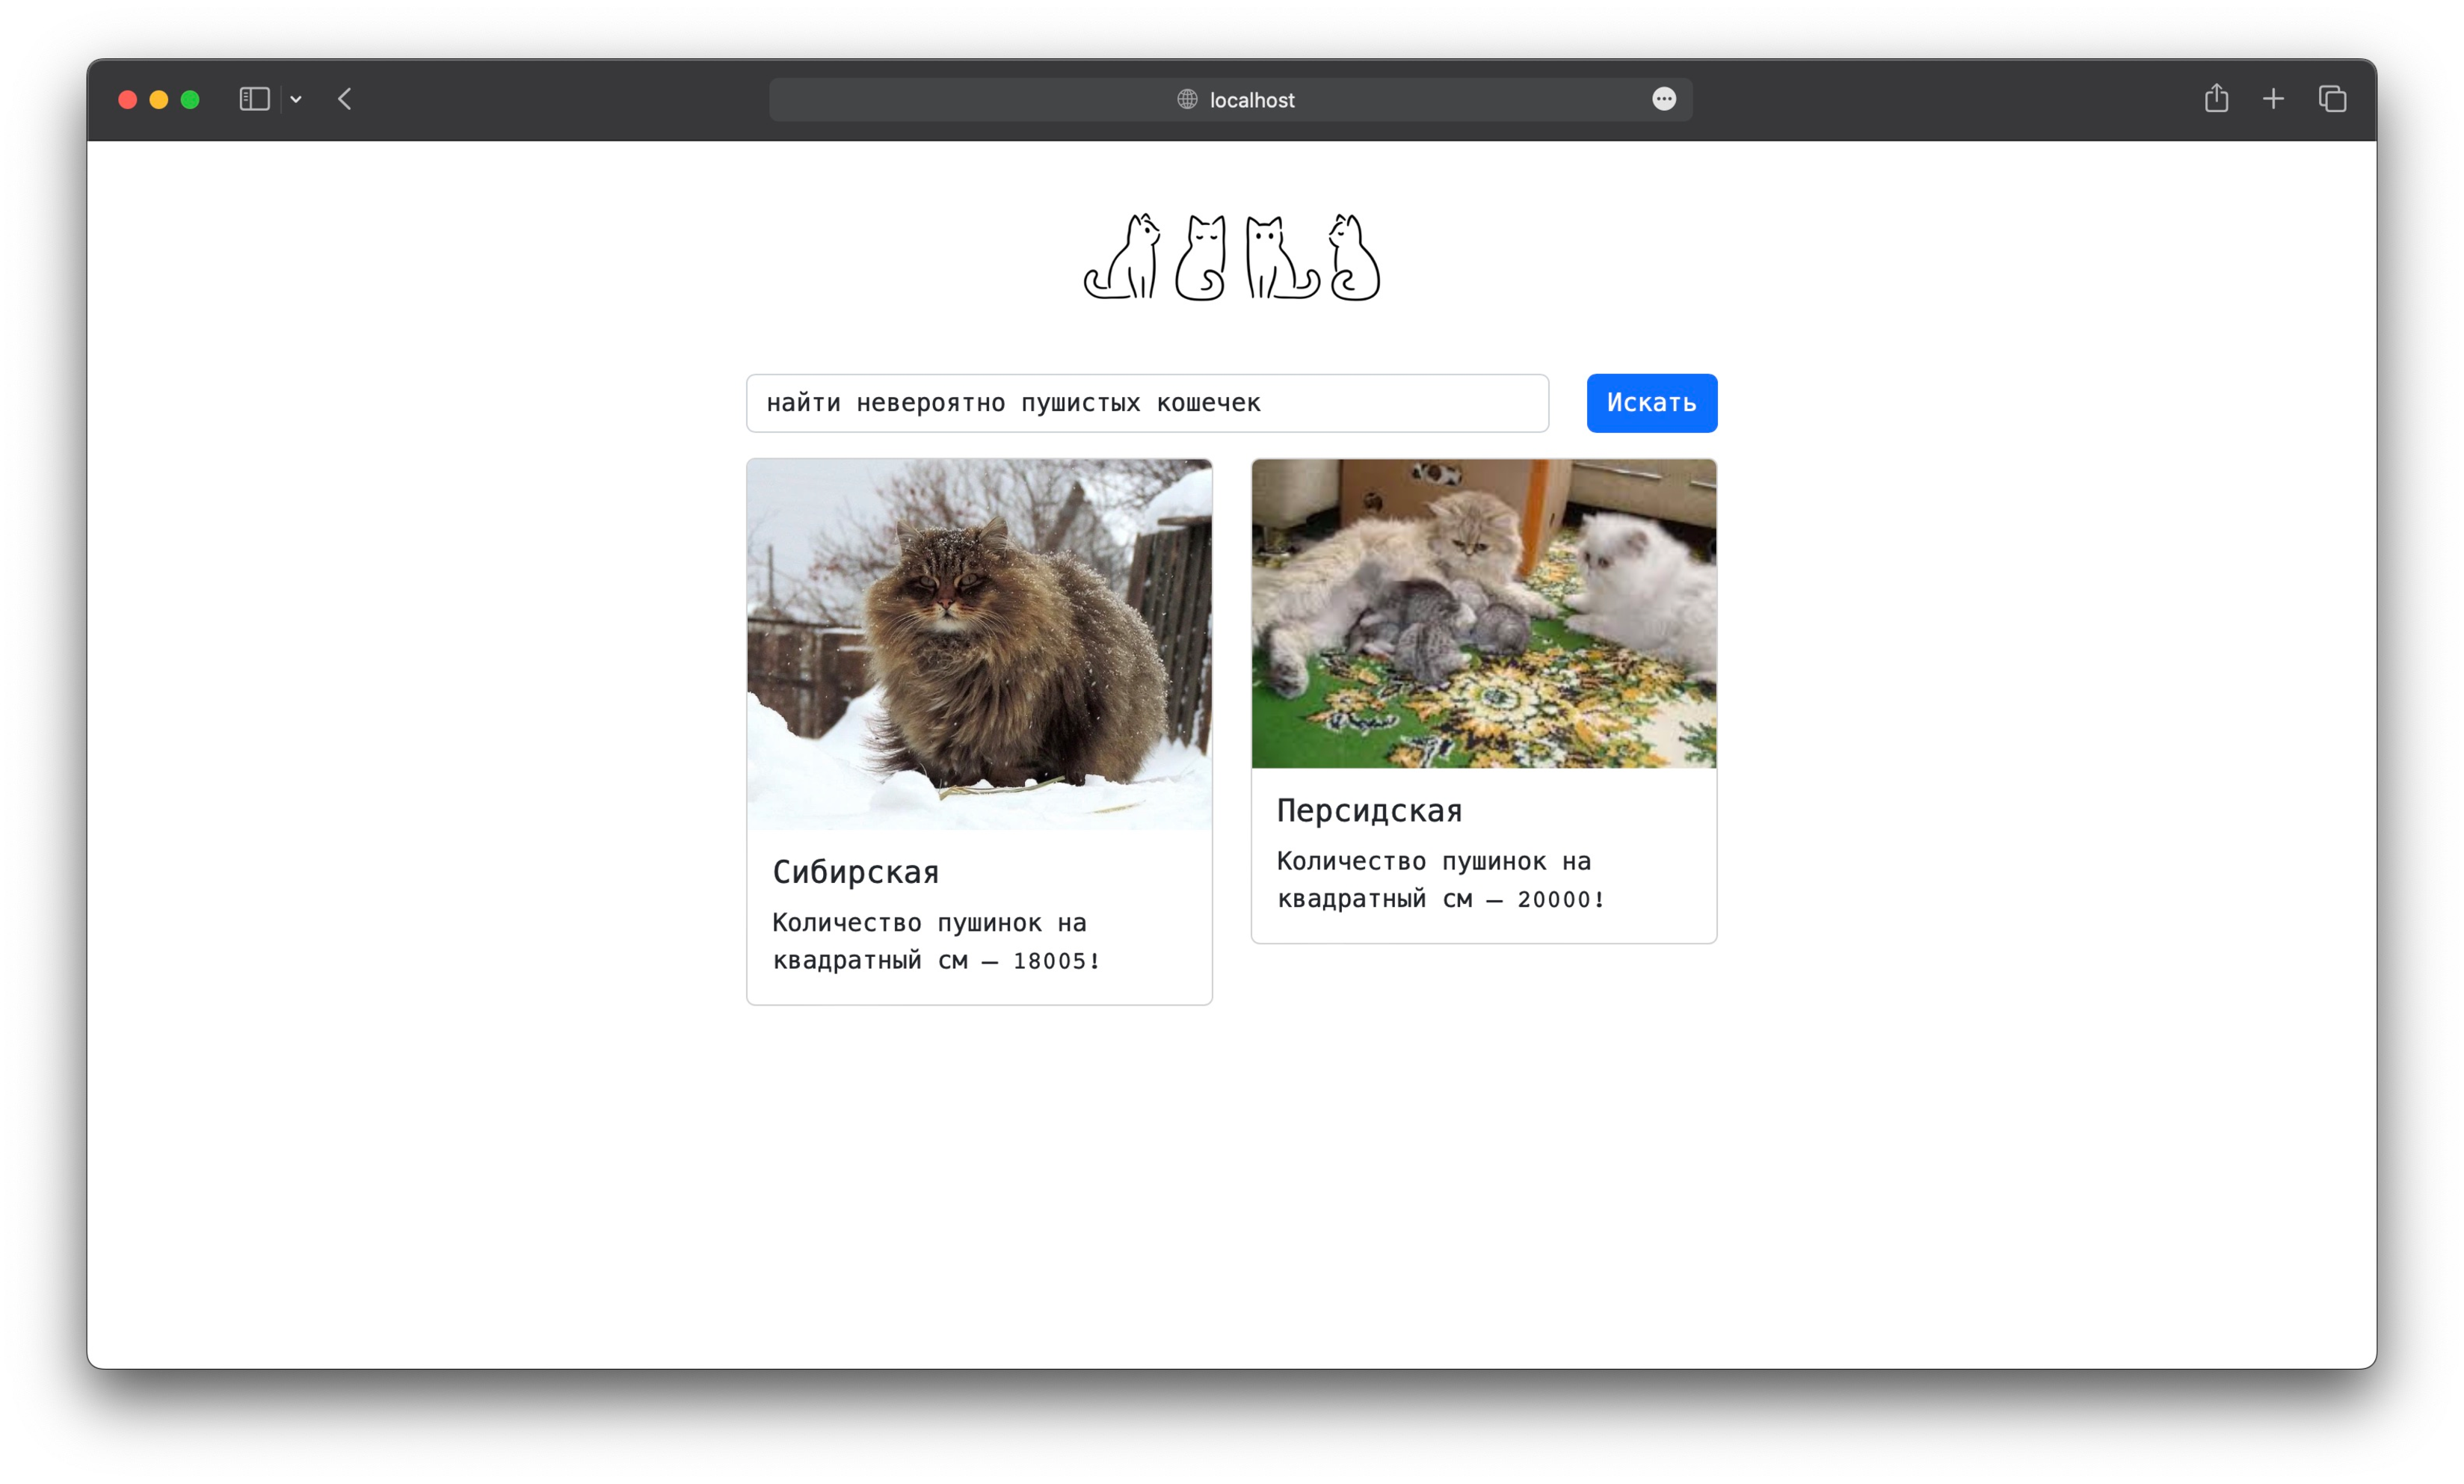
\includegraphics[width=0.37\linewidth]{int2.pdf}
    \caption{Разность фаз волн света в мыльной пленке}
    \label{img:int2}
\end{figure}

Геометрическая разница в расстоянии составляет $AB + BC - AJ$. Свет всегда распространяется медленнее в более плотной среде, поэтому расстояние, пройденное светом в мыльной плёнке, нужно умножить на показатель преломления мыльной воды. Таким образом, эта часть разности хода составляет 
\begin{equation} \label{eqn:1}
	\Delta = \eta(AB + BC) - AJ. 
\end{equation}

По рисунку видно, что:
\begin{equation}
	\cos(\theta_t) = \frac{w}{AB},
\end{equation}
\begin{equation}
	AB = BC.
\end{equation}
Тогда
\begin{equation}
	AB = BC = \frac{w}{\cos(\theta_t)}.
\end{equation}

После подставления результата в формулу (\ref{eqn:1}) получается
\begin{equation}
	\Delta = 2 \cdot \eta \cdot \frac{w}{\cos(\theta_t)} - AJ.
\end{equation} 

Так как $\angle{ACJ} = \theta_i$, то $AJ = AC \cdot \sin(\theta_i)$. По закону Снеллиуса $AJ = AC \cdot \eta \cdot \sin(\theta_t)$. Также видно, что $\tan(\theta_t) = \frac{\frac{AC}{2}}{w}$, поэтому $AC = 2 \cdot w \ cdot \tan(\theta_t)$.

После подставления результата в формулу (\ref{eqn:1}) получается
\begin{equation}
	\Delta = 2 \cdot \eta \cdot \frac{w}{\cos(\theta_t)} - 2 \cdot w \cdot \tan(\theta_t) \cdot \eta \cdot \sin(\theta_t).
\end{equation} 

Если упростить данное выражение, то получится
\begin{equation}
	\Delta = 2 \cdot w \cdot \eta \cdot \cos(\theta_t).
\end{equation}

Также известно, что, когда свет переходит из одной среды в среду с более высоким показателем преломления, он претерпевает фазовый сдвиг, равный половине длины его волны, то есть $\frac{\lambda}{2}$. 

Тогда итоговая разность хода
\begin{equation}
	\Delta_{res} = 2 \cdot w \cdot \eta \cdot \cos(\theta_t) - \frac{\lambda}{2}.
\end{equation}

Если в разность хода укладывается чётное число полуволн, то в точке падения луча будет максимум интенсивности света. Если в разность хода укладывается нечётное число полуволн, то в точке падения луча будет минимум интенсивности света.

По данной формуле рассчитывается разность фаз:
\begin{equation}
	\delta = \frac{2 \cdot \pi \cdot \Delta_{res}}{\lambda}.
\end{equation}

Для волн с одинаковой интенсивностью итоговая интенсивность в результате интерференции будет рассчитываться по формуле
\begin{equation}
	I = 2 \cdot I_0 \cdot (1 + \cos(\delta)).
\end{equation}

\section{Выводы по аналитической части}
В данном разделе были проведены анализ и формализация объектов синтезируемой сцены, исследование задачи построения реалистичного трёхмерного изображения сцены из данных объектов, и рассмотрены различные методы, решающие перечисленные задачи.

\newpage